% \section{Software Requirements Specification}

\section{Einführung}

\subsection{\textbf{Zweck}}
Dieses Dokument dient als Dokumentation des berufsbegleitenden Studienganges, Kommunikations- und Medieninformatik des Matrikel 13, mit der Programmierung einer APP zur Kompression von Bilddaten. Es setzt dabei die Rahmenbedingungen fest.

%\subsection{\textbf{Hintergründe und Ziele des Projekts}}
%Die \acf{HfTL} ist eine private, staatlich anerkannte Fachhochschule. Träger der \ac{HfTL} ist die \ac{HfTL}-Trägergesellschaft \acs{mbH}, eine Beteiligungsgesellschaft der Deutschen Telekom AG. Die Hochschule befindet sich im Leipziger Stadtteil Connewitz. Es werden sowohl Direkt- als auch duale Studiengänge und berufsbegleitende Studiengänge angeboten.

\subsection{\textbf{Produktanforderungen}}

Der Betrieb der Smartphone-APP muss auf allen gängigen Android-Smartphones ab Version 4.4.2 möglich sein.

Durch die APP wird den Studenten der HFTL ermöglicht: 

\begin{itemize}
      \item Fotos aufnehmen
      \item Bilder mit einer skalaren Quantisierung komprimieren
      \item Quantisierungsinterval soll einstellbar sein 
      \item Ablage der komprimierten Bilder in passend zum Verfahren benannten Ordnern
\end{itemize}
   



\subsection{\textbf{Musskriterien}}

Zunächst müssen zwingend folgende Punkte des Umfangs erfüllt werden:

\begin{itemize}
   	\item Bildaufnahme
   	\item Quantisierung
   	\item Auswahl Quantisierungsinterval
   	\item Abspeichern mit passendem Dateinamen 
\end{itemize}

%\subsection{\textbf{Abgrenzungskriterien}}
%
%Die \acs{APP} soll später auch um zusätzliche Funktionen, wie Vektorquantisierung oder andere Verfahren erweiterbar sein. Versionen für andere Betriebssysteme müssen in einem seperaten Projekt bearbeitet werden und sind nicht Bestandteil dieses Projektes.			

\subsubsection{Kostenrahmen}

Für die Entwicklung der \acs{APP} soll auf kostenfreie Opensource-Programme oder auf vordefinierte Klassen für die Programmierung zurückgegriffen werden.


\subsection{\textbf{Definitionen, Akronyme, Abkürzungen}}
\begin{acronym}[UV-Licht]
\acro{HfTL}{Hochschule für Telekommunikation Leipzig}
\acro{APP}{Kurzform für Applikation}
\acro{mbH}{mit beschränkter Haftung}
\acro{QIS}{Qualitätssteigerung der Hochschulverwaltung im Internet durch Selbstbedienung}
\acro{iCal}{Datenformat zum Austausch von Kalenderinhalten}
\acro{SoSe15}{Sommersemester 2015}
\acro{XML}{ Extensible Markup Language}
\acro{HTTPS}{HyperText Transfer Protocol Secure}
\acro{AES}{Advanced Encryption Standard}
\acro{SQL}{Structured Query Language}
\acro{.apk}{Android application package}
\acro{MTBF}{mean time between failure}
\acro{CI/CD}{Corperate Identity/Corperate Design}
\acro{GUI}{Graphical User Interface}
\acro{QuantiPig}{quantisiertes Picture}


\end{acronym}

%\subsection{\textbf{Referenzen}}
%
%\begin{itemize}		
%	\item QIS-System:  \url{https://qisweb.hispro.de/tel/rds?state=user&type=0} 
%	
%	\item News der HfTL  \url{https://www.hft-leipzig.de/de/studierende/service/news.html}	
%\end{itemize}


\section{Allgemeine Übersicht}

\subsection{\textbf{Beschreibung der Ausgangssituation (Ist-Zustand) }}

Als Ausgangssituation wurden der Studentengruppe drei \acs{APP}'s aus vorherigen Matrikeln vorgelegt, die ebenfalls Bilddaten komprimieren. Diese drei \acs{APP}'s gilt es zu vergleichen und die Stärken herauszuarbeiten. Anhand dieser Ergebnisse gilt es eine neue \acs{APP} zu entwickeln.


\subsubsection{Vergleich der vorhandenen drei \acs{APP}'s}
\begin{landscape}

\newpage

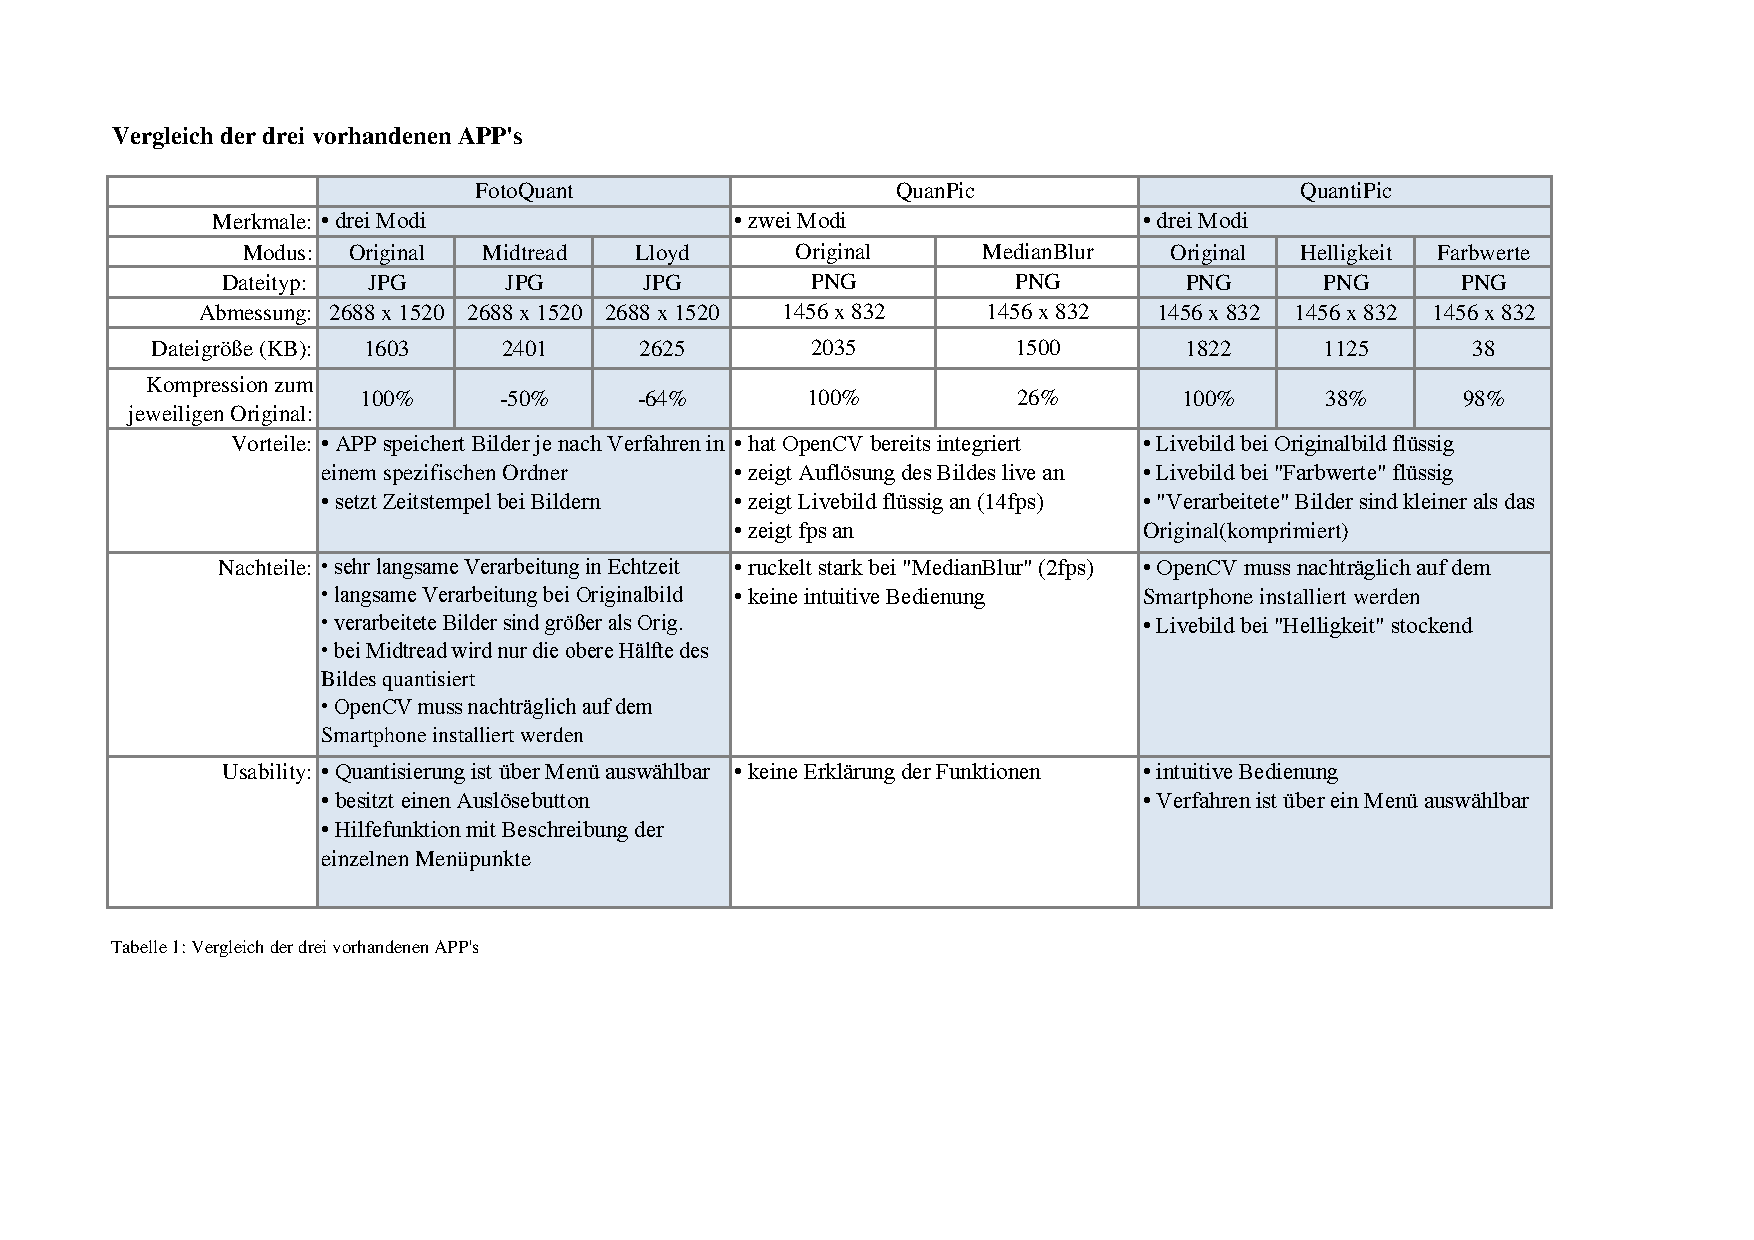
\includepdf[landscape=true,pages=-,noautoscale]{04_Anhang/files/Vergleich_Apps.pdf}


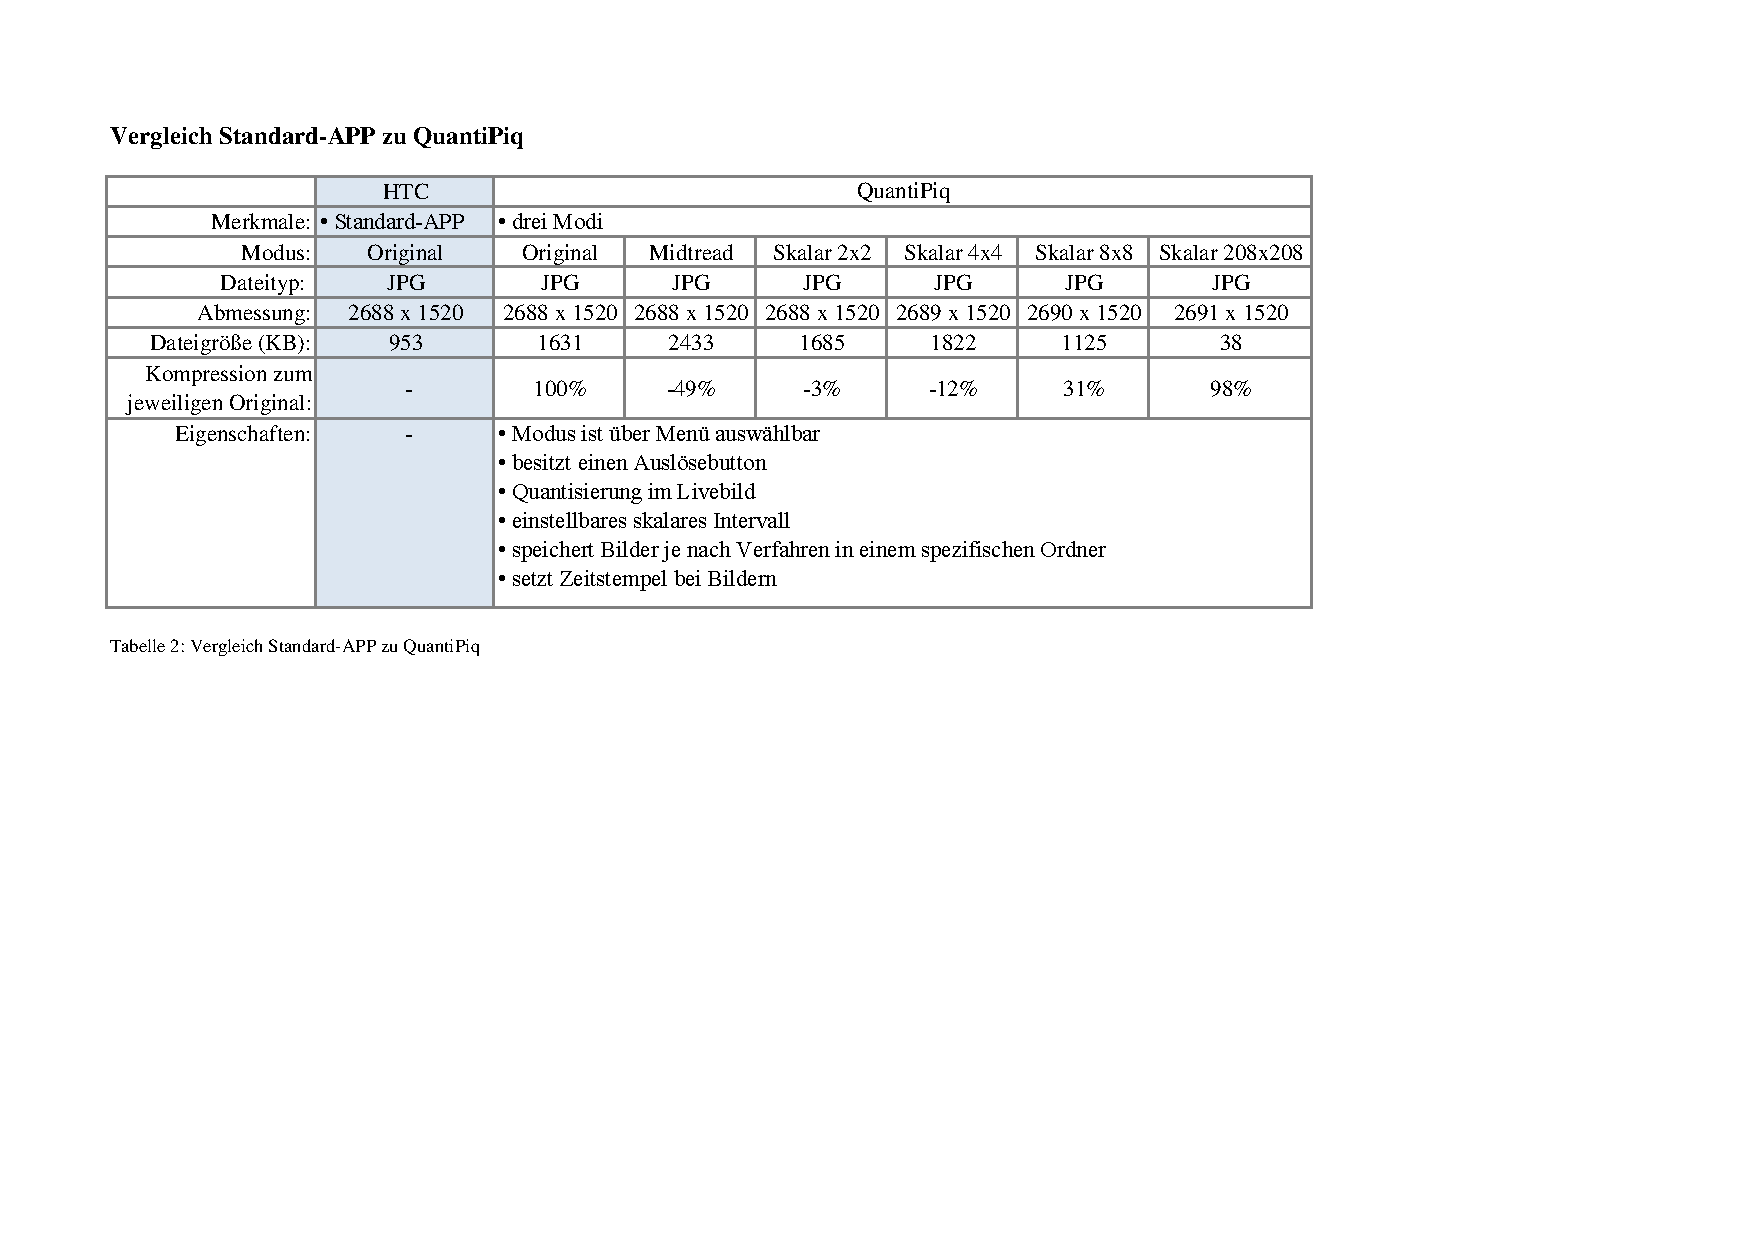
\includepdf[landscape=true,pages=-,noautoscale]{04_Anhang/files/Vergleich2.pdf}

\end{landscape}


\subsection{Beispielbilder}

\begin{landscape}

\begin{figure}[h]
	\centering
		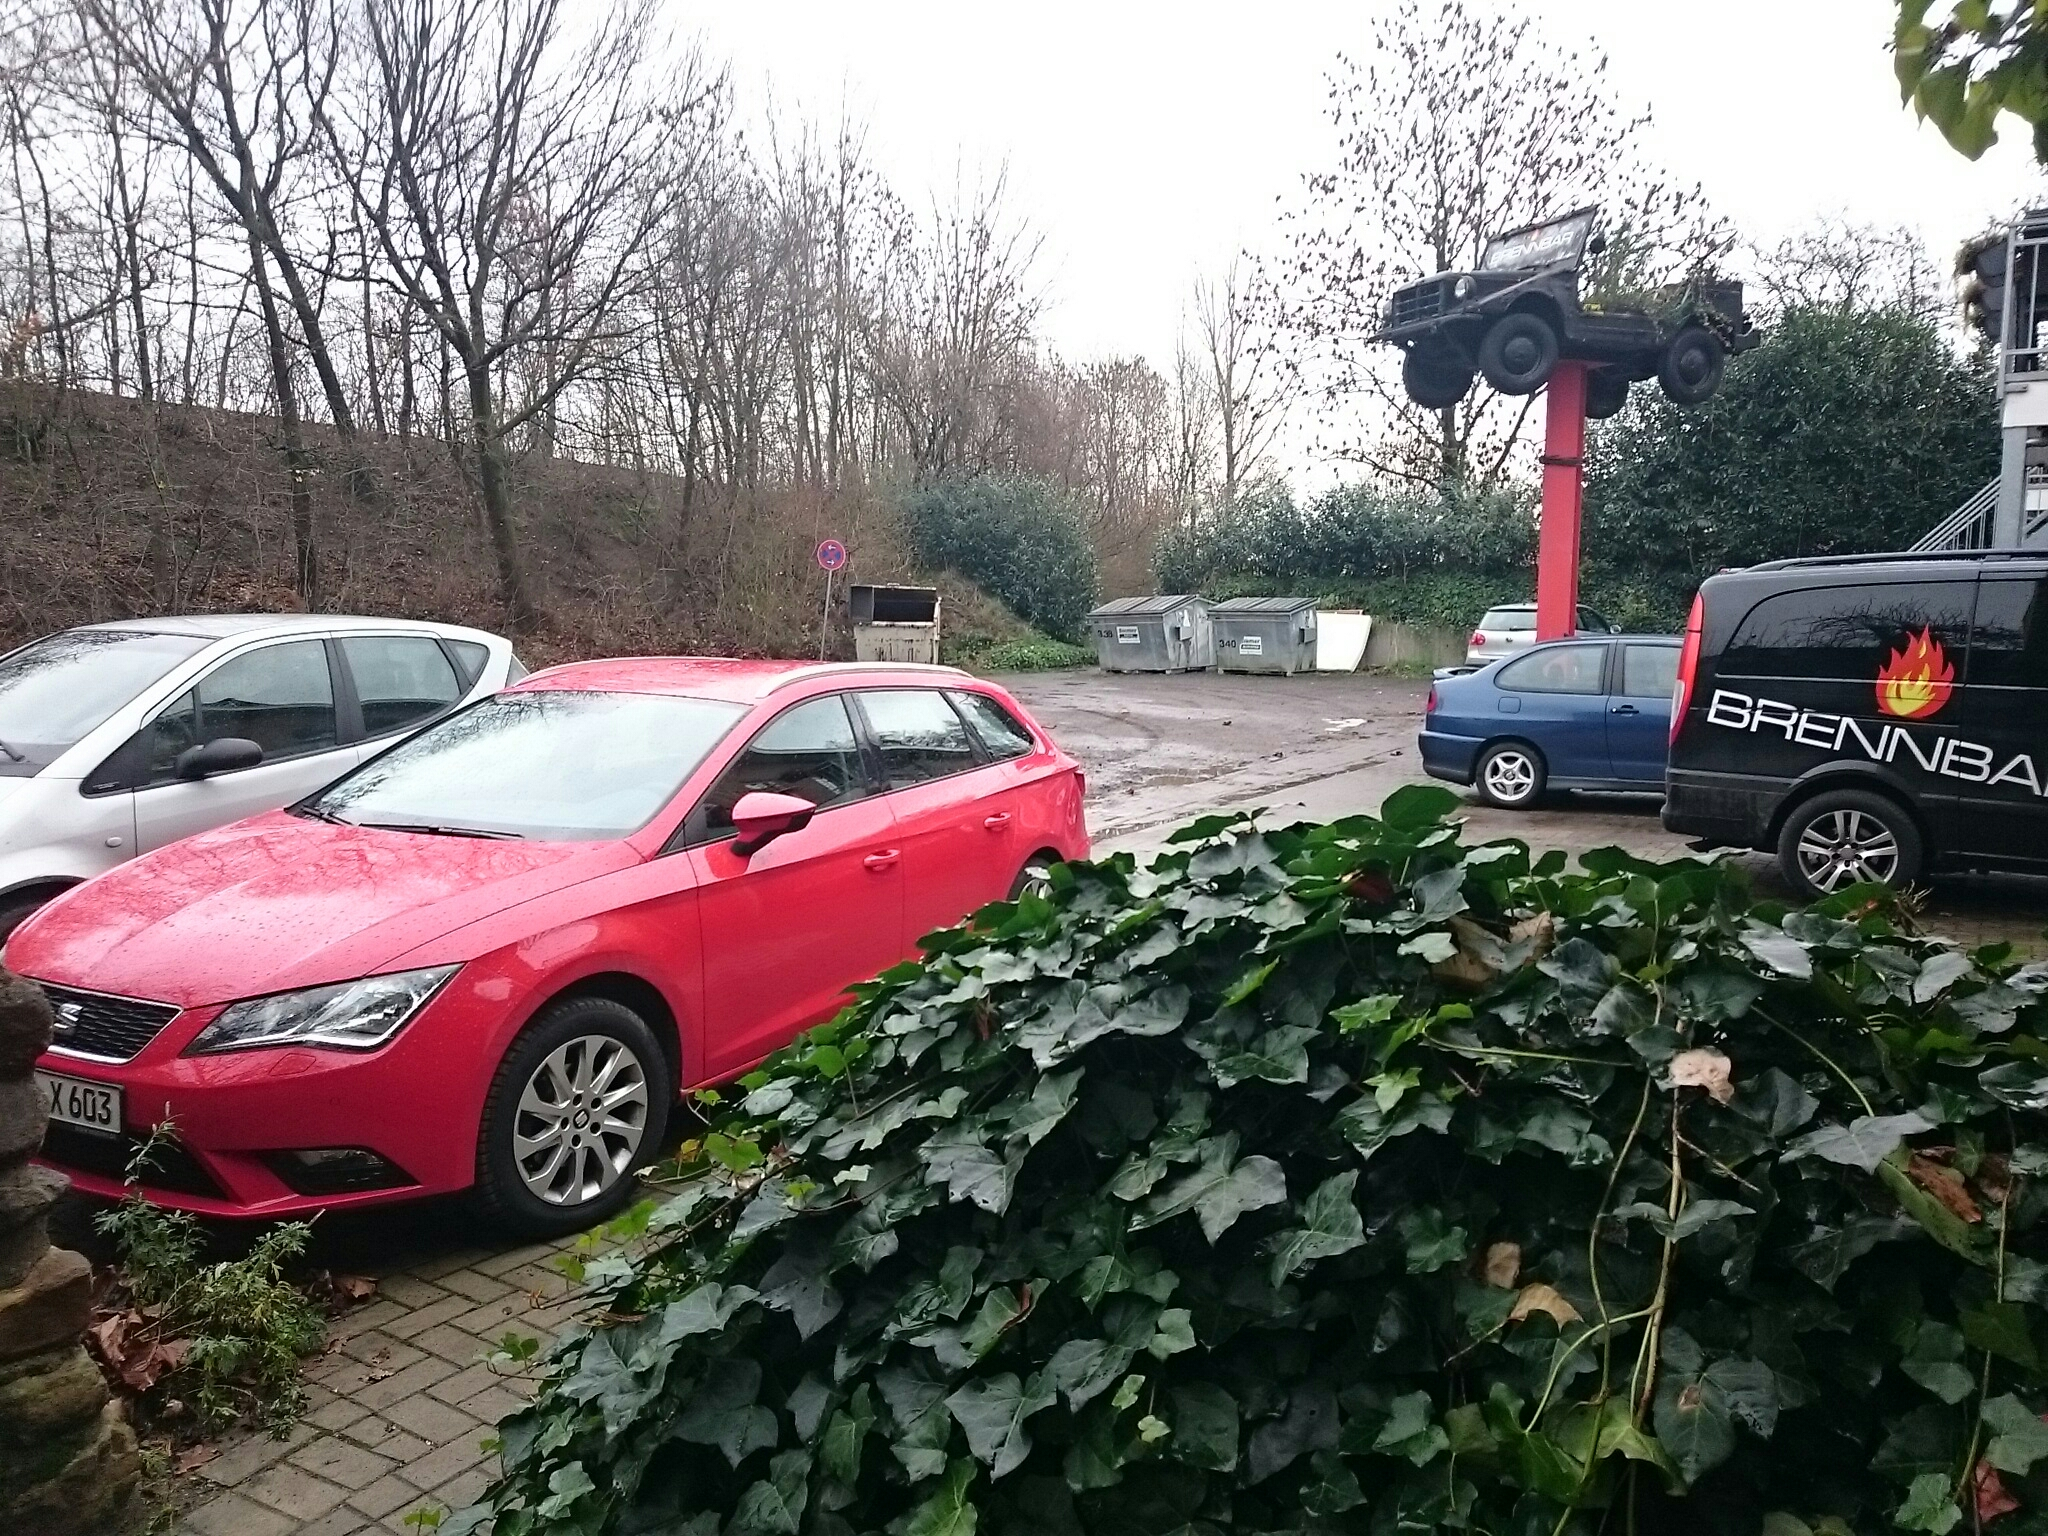
\includegraphics[width=1.4\textwidth]{img/Fotos/FotoQuant_Original.jpg}
	\caption[FotoQuant Original]{FotoQuant Originalbild}
	\label{fig:quant_ori}
\end{figure}

\begin{figure}[h]
	\label{fig:quant_mid}
	\centering
		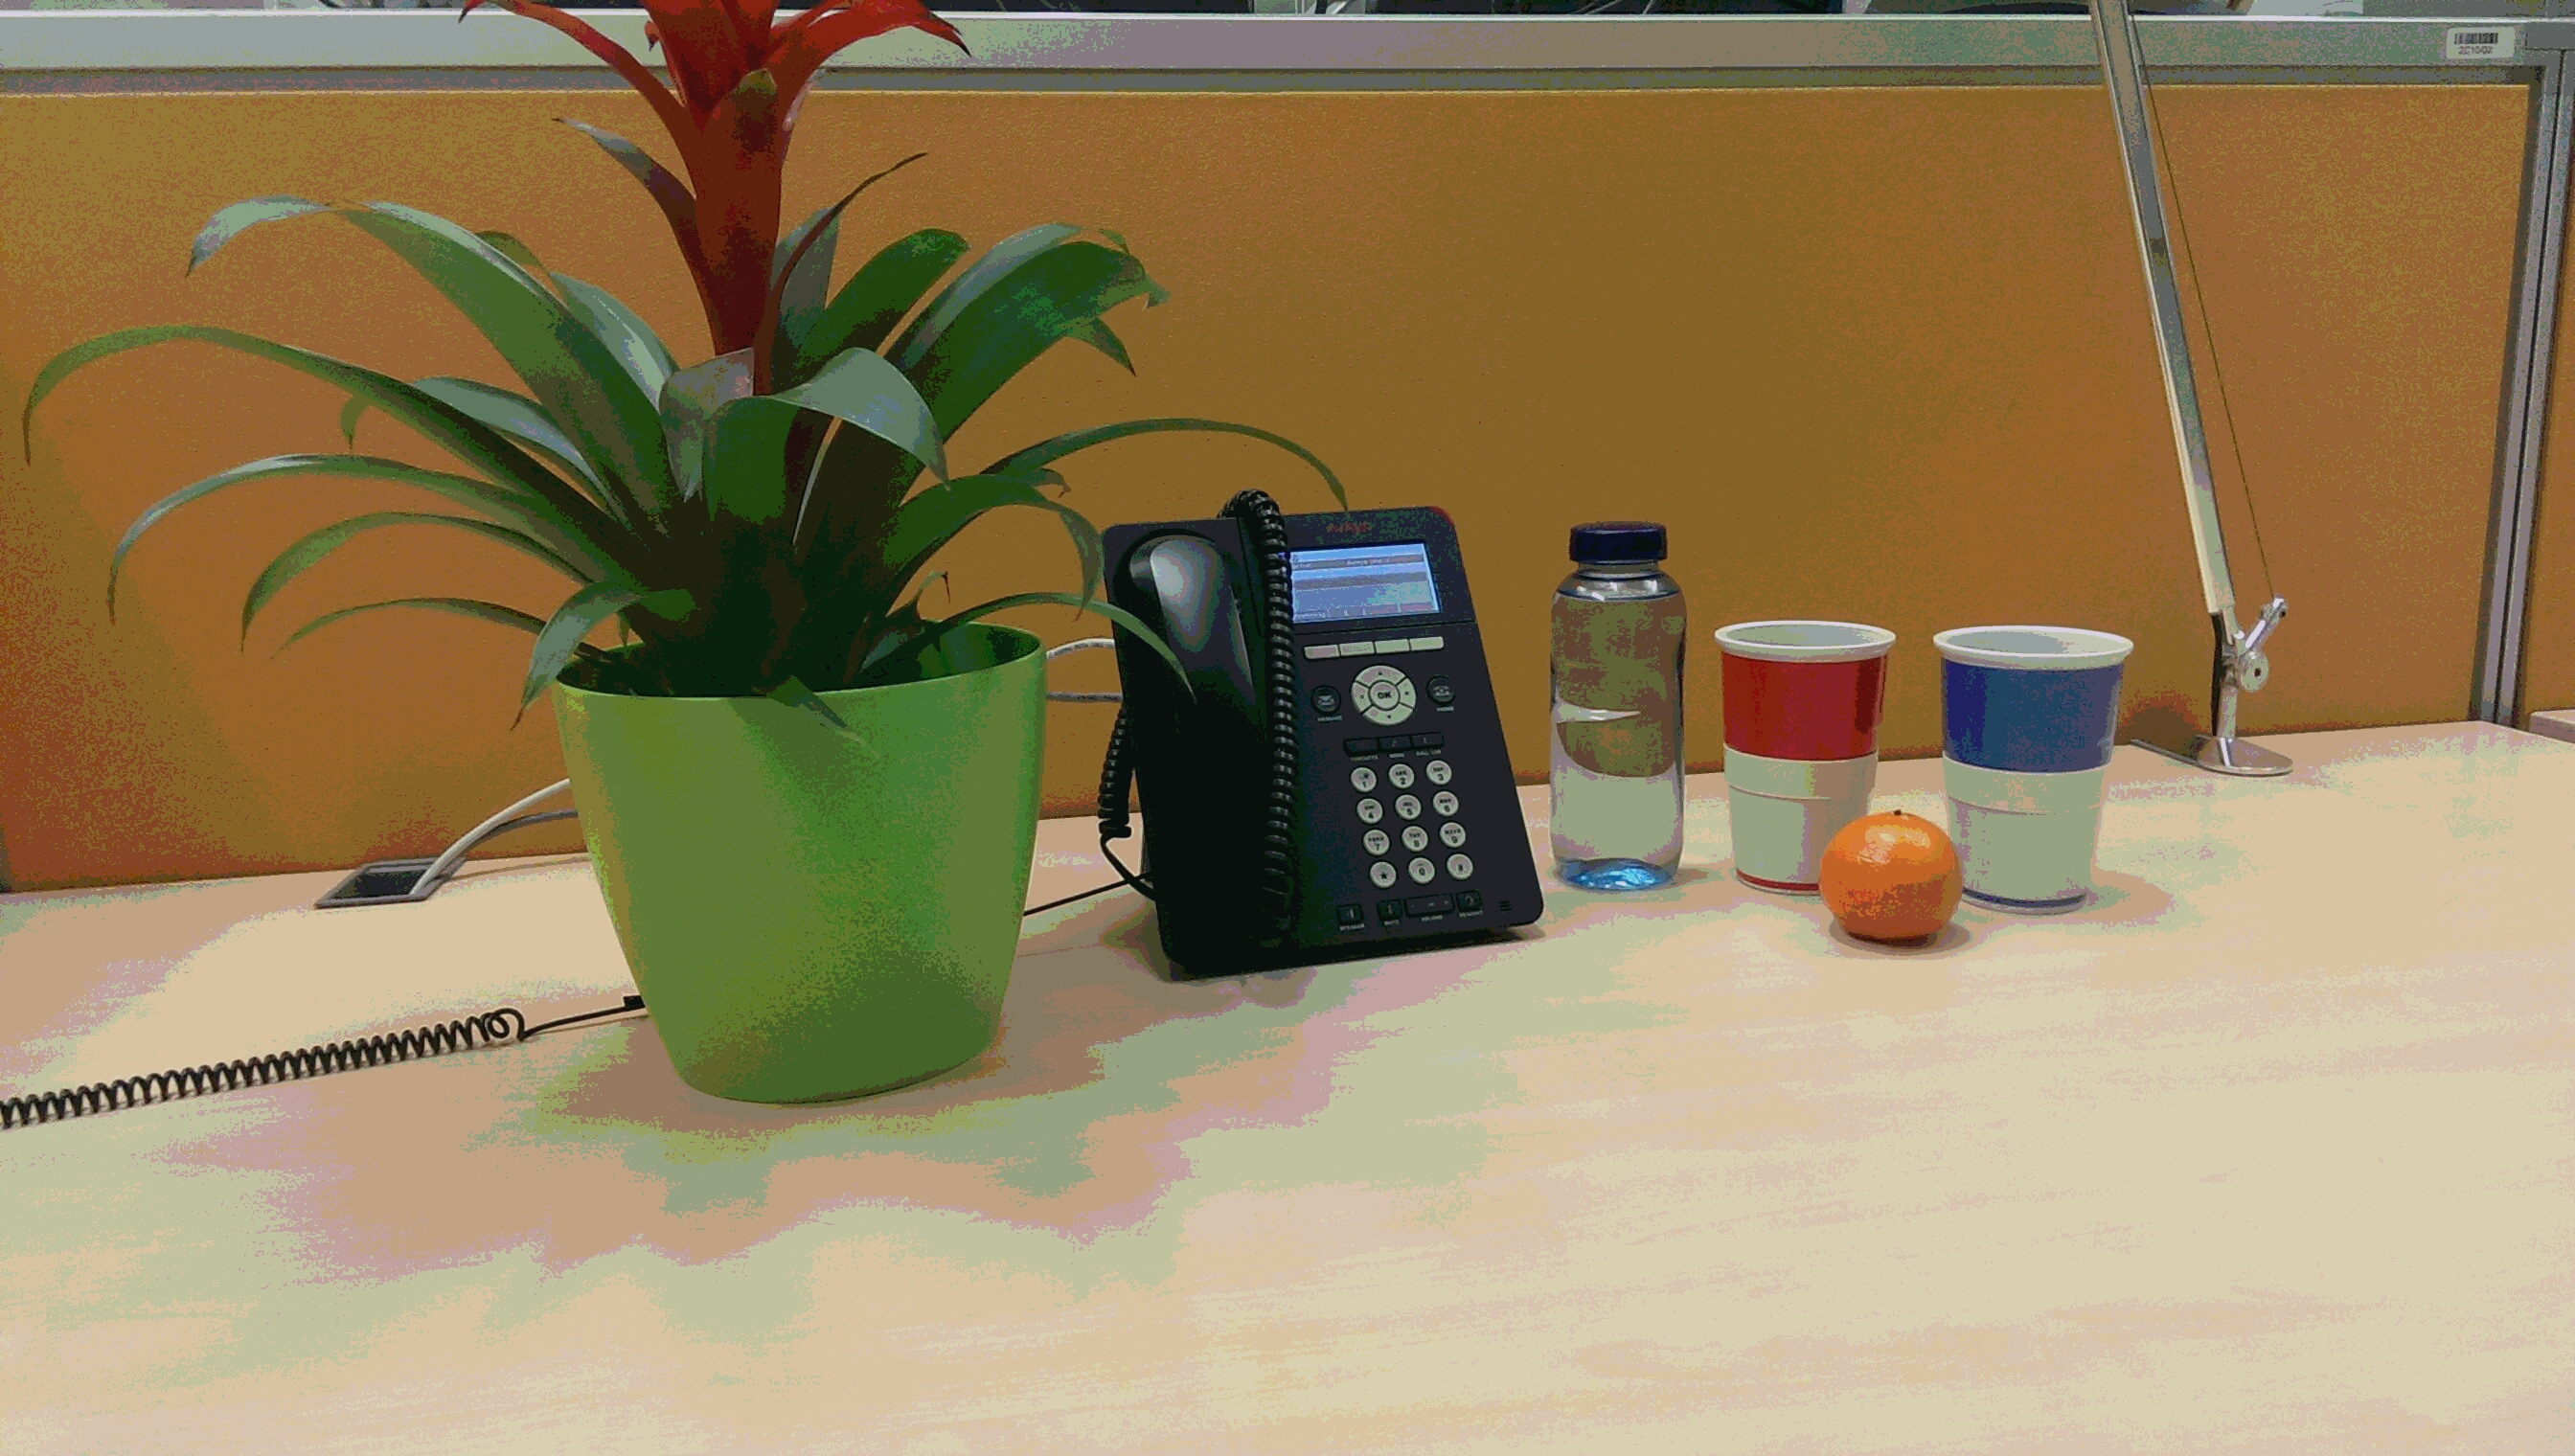
\includegraphics[width=1.4\textwidth]{img/Fotos/FotoQuant_Lloyd.jpg}
	\caption[FotoQuant Lloyd]{FotoQuant Lloyd-Modus}
	\label{fig:quant_lloyd}
\end{figure}

\begin{figure}[h]
	\centering
		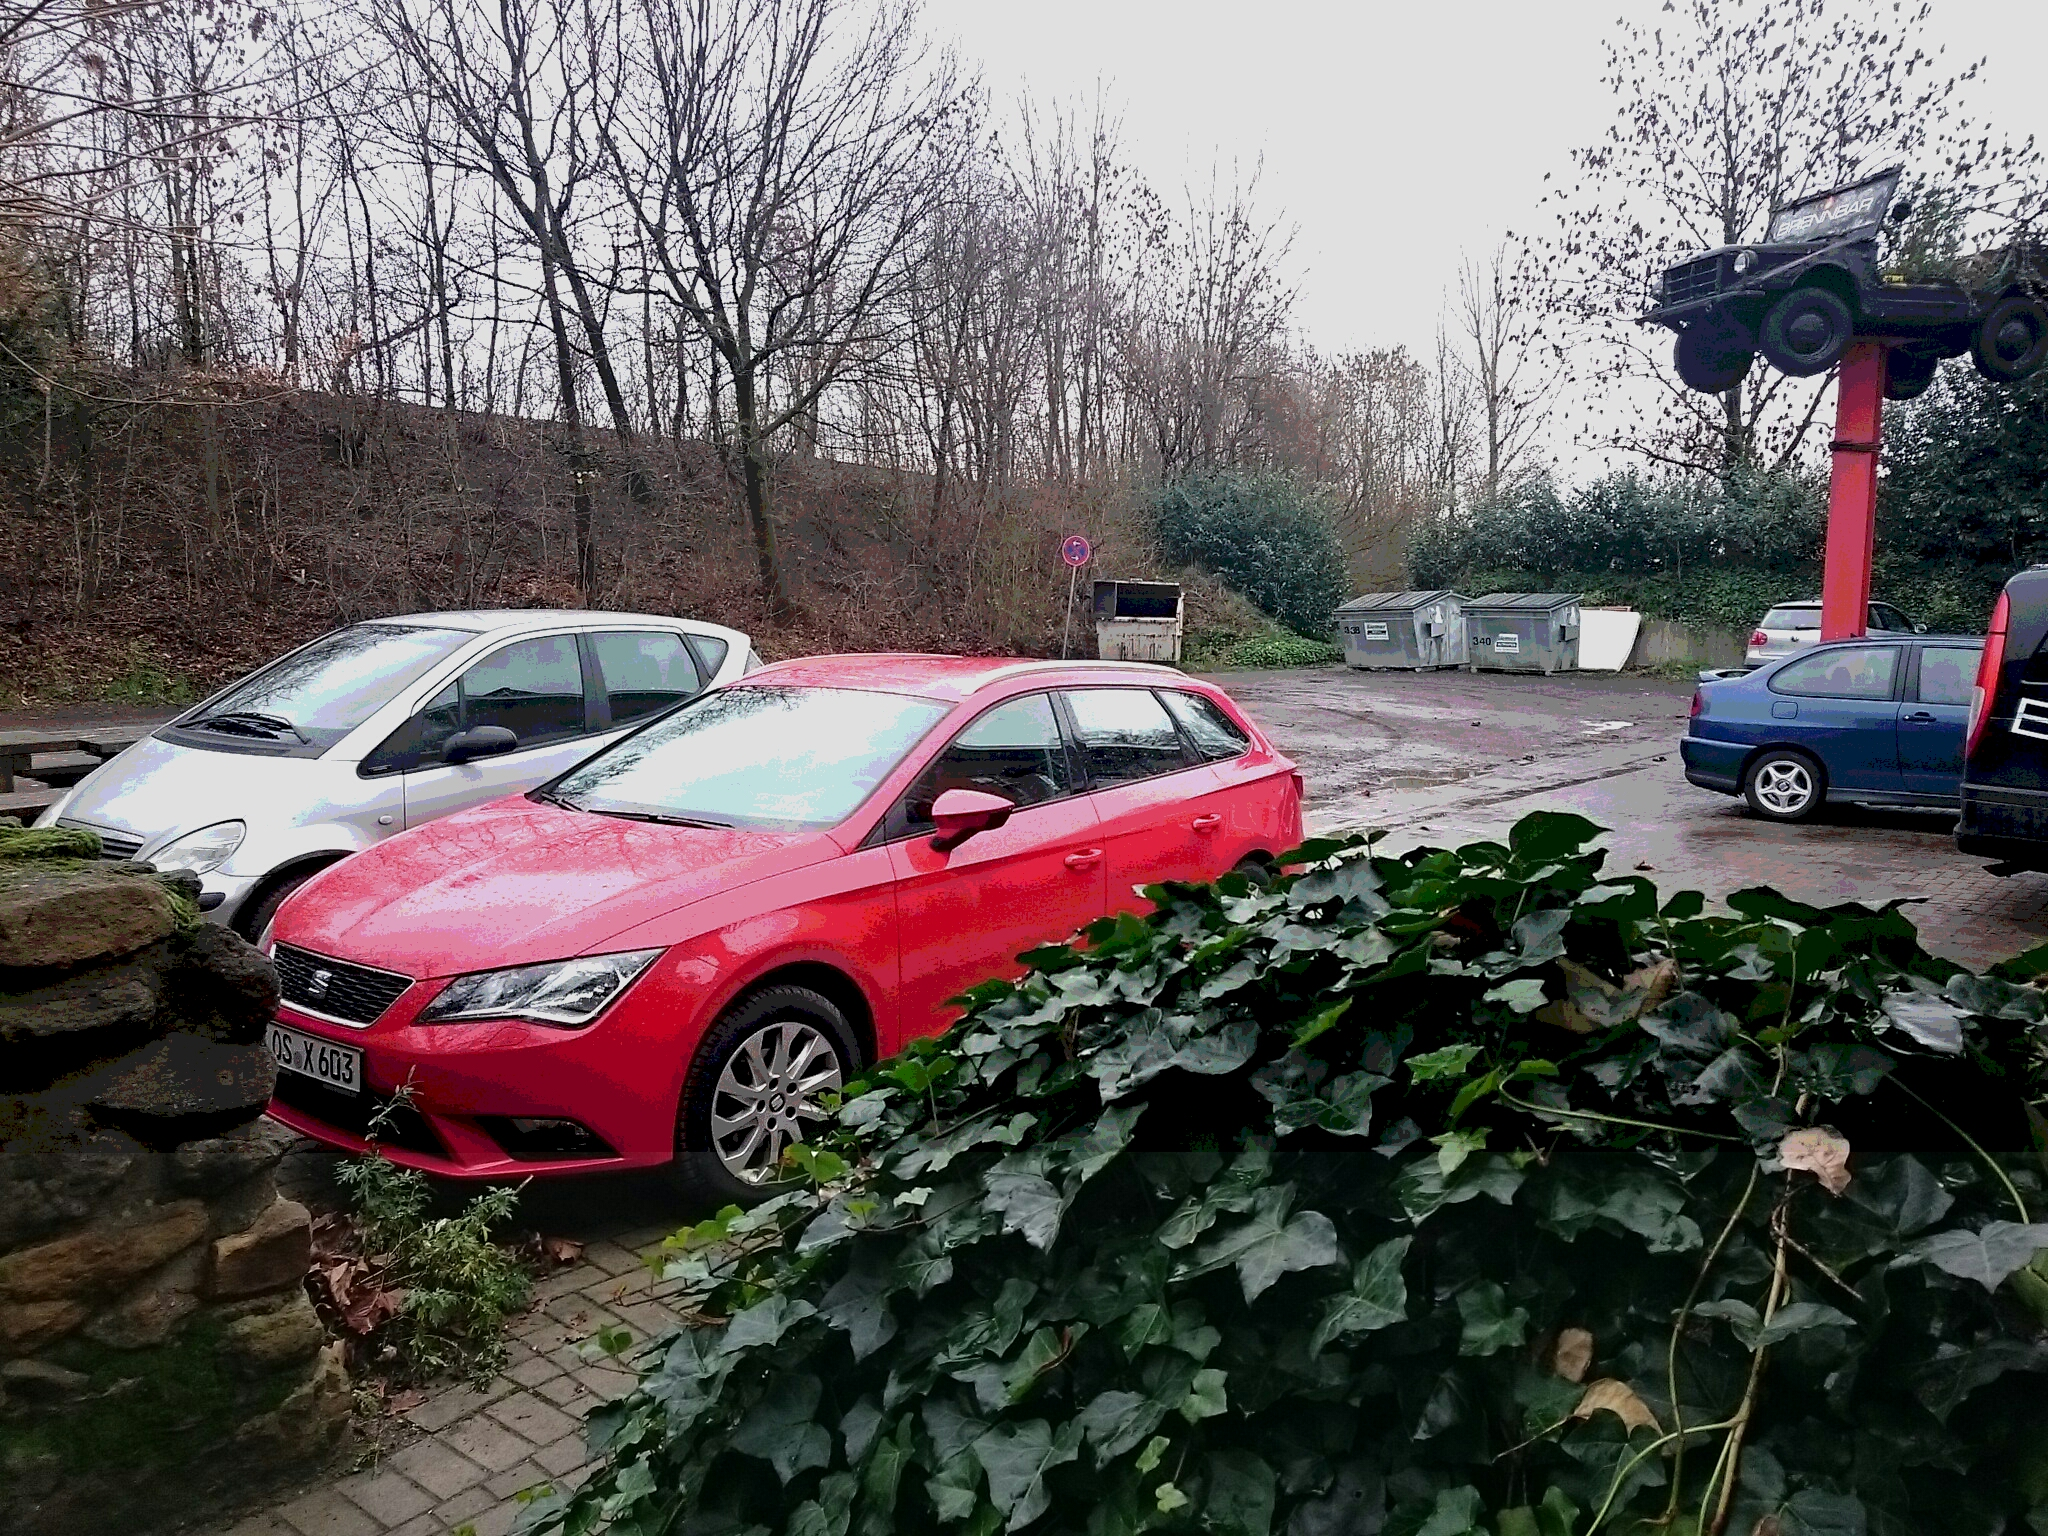
\includegraphics[width=1.4\textwidth]{img/Fotos/FotoQuant_Midtread.jpg}
	\caption[FotoQuant MidTread]{FotoQuant MidTread-Modus}
	\label{fig:quant_mid}
\end{figure}

\begin{figure}[h]
	\centering
		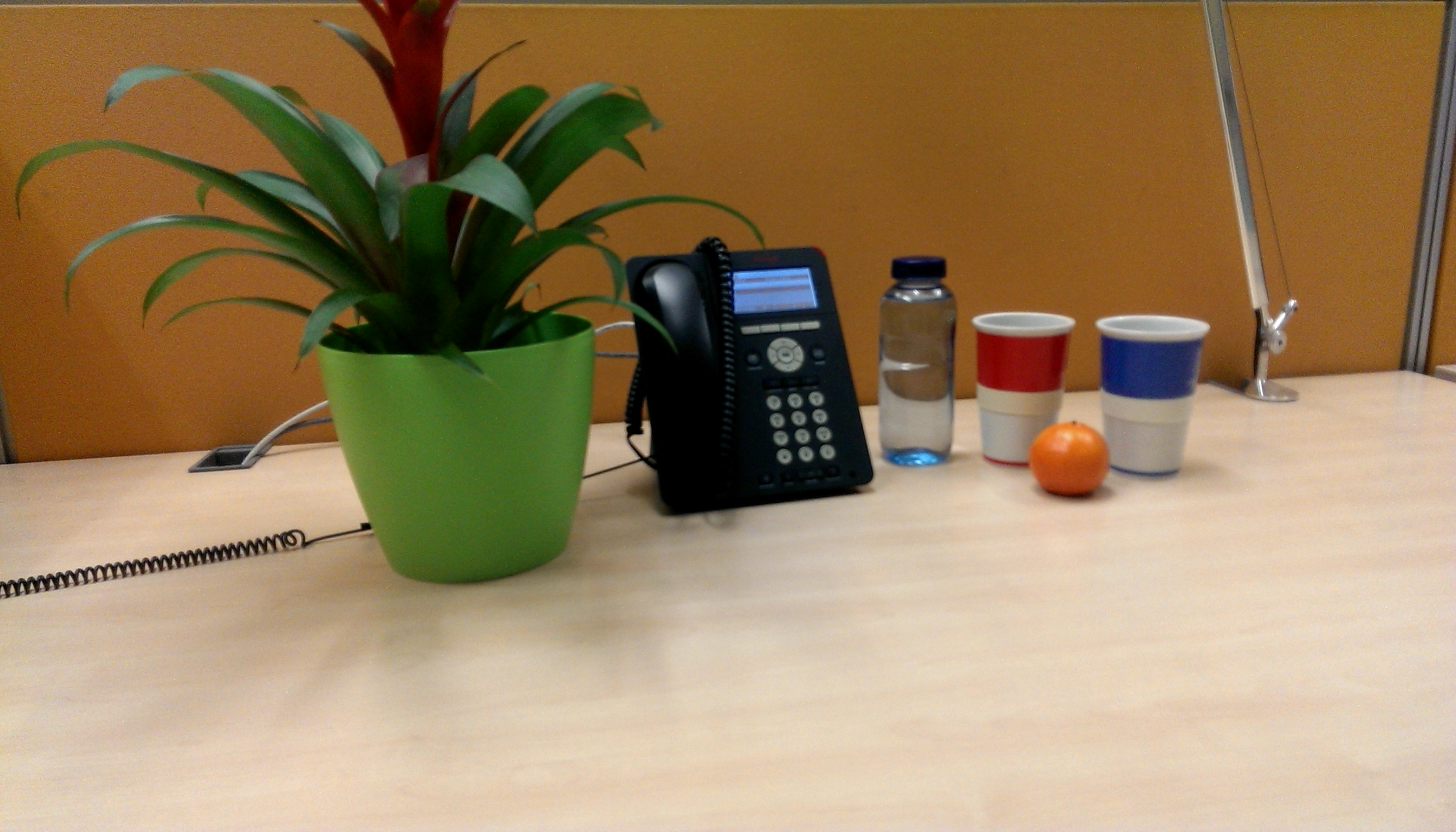
\includegraphics[width=1.4\textwidth]{img/Fotos/QuanPic_Original.png}
	\caption[QuanPic Original]{Quanpic im Originalbild-Modus}
	\label{fig:quan_orig}
\end{figure}

\begin{figure}[h]
	\centering
		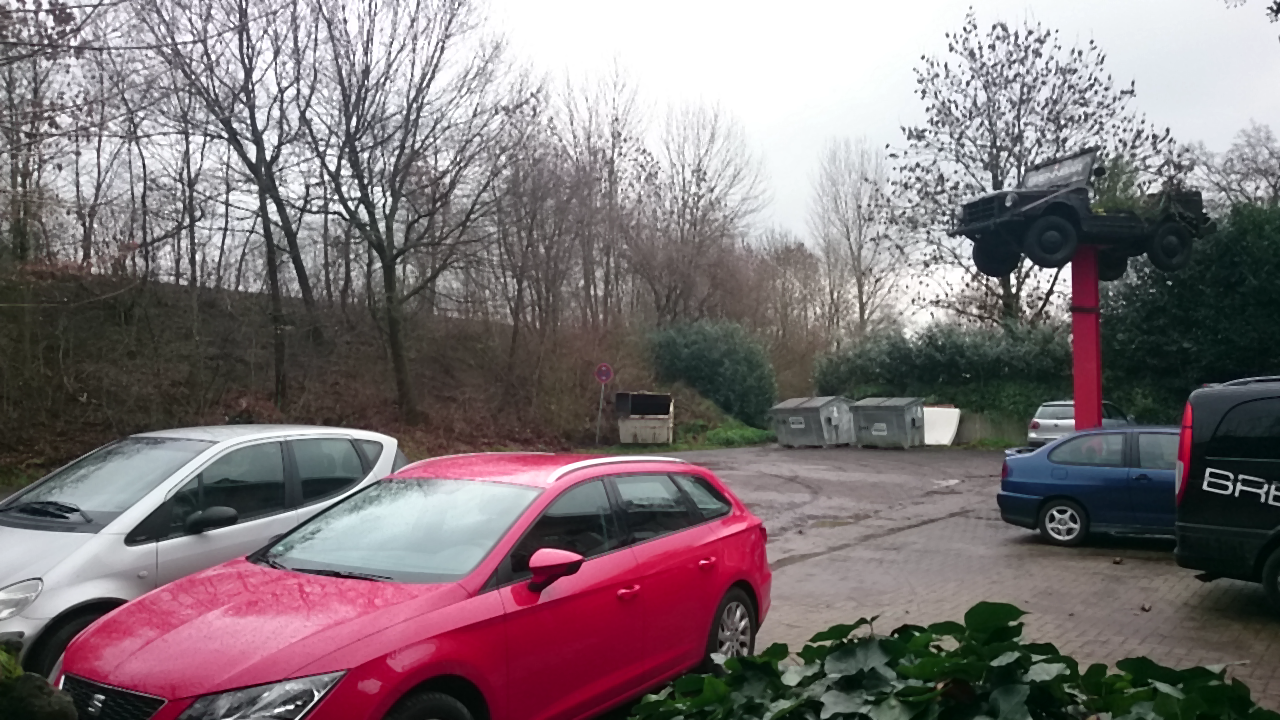
\includegraphics[width=1.4\textwidth]{img/Fotos/QuanPic_Medianblur.png}
	\caption[QuanPic MedianBlur]{Quanpic im MedianBlur-Modus}
	\label{fig:quan_med}
\end{figure}

\begin{figure}[h]
	\centering
		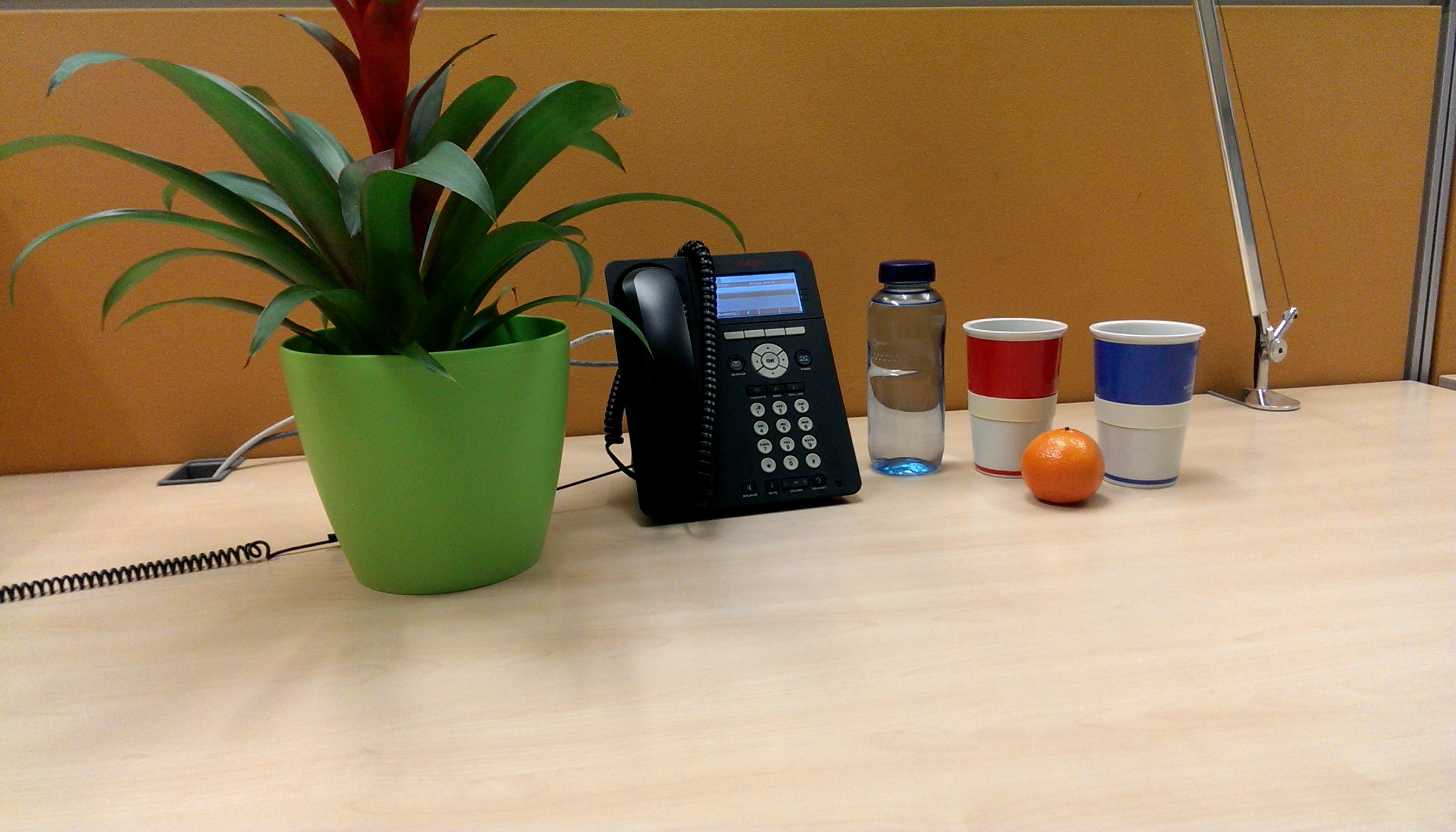
\includegraphics[width=1.4\textwidth]{img/Fotos/QuantiPic_Original.png}
	\caption[QuantiPic Originalbild]{QuantiPic im Originalbild-Modus}
	\label{fig:quanti_orig}
\end{figure}

\begin{figure}[h]
	\centering
		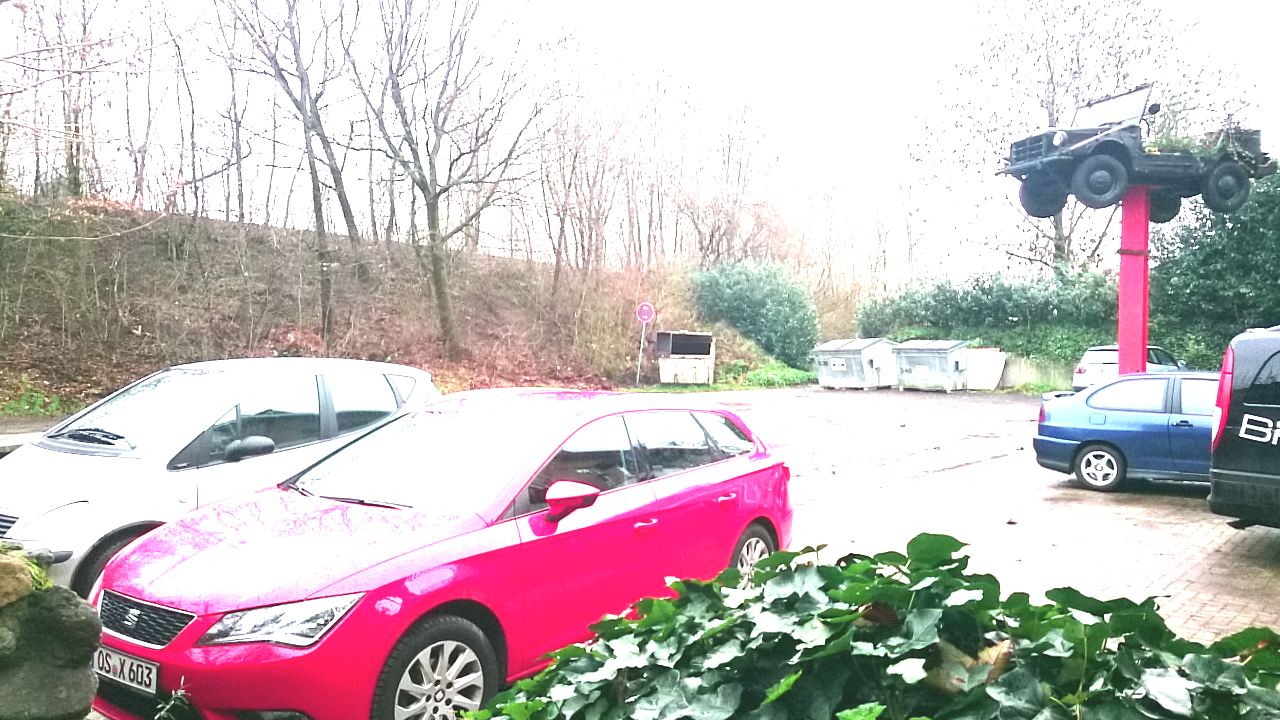
\includegraphics[width=1.4\textwidth]{img/Fotos/QuantiPic_Helligkeit.png}
	\caption[QuantiPic Helligkeit]{QuantiPic im Helligkeits-Modus}
	\label{fig:quanti_hell}
\end{figure}

\begin{figure}[h]
	\centering
		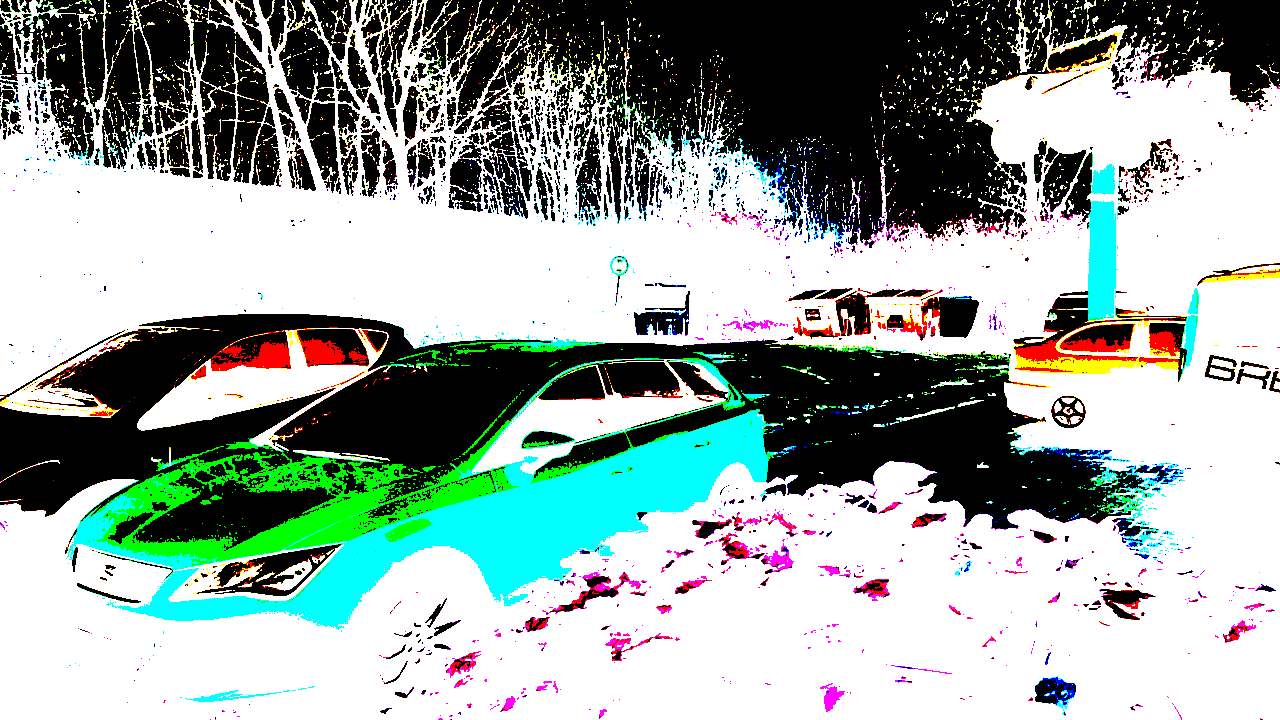
\includegraphics[width=1.4\textwidth]{img/Fotos/QuantiPic_Farbwerte.png}
	\caption[QuantiPic Farbwerte]{QuantiPic im Farbwerts-Modus}
	\label{fig:quanti_farb}
\end{figure}





\end{landscape} 

\subsection{\textbf{Produkteinsatz}}

\subsubsection{Anwendungsbereiche}
Aktuell soll die APP nur für die Studenten der \acs{HfTL} zugänglich sein, welche ein Android-Smartphone besitzen. 

\subsubsection{Zielgruppen, Qualifikationsniveau}

Da bei der Nutzergruppe von Studenten mit Erfahrung im Umgang mit solchen APP's ausgegangen werden kann, wird auch die Oberfläche dementsprechend gestaltet.

\subsection{\textbf{Produktfunktionalität}}

Auszug aus der Aufgabenbeschreibung:

\textit{\glqq
Auf Basis der Analyse ist eine neue App zu programmieren,
welch die positiven Eigenschaften der vorhandenen Apps vereint und als Verarbeitungsfunktion
das Bild gleichmäßig mit einem einstellbaren Quantisierungsintervall quantisiert.\grqq
} 

\subsection{\textbf{Randbedingungen}}

Der zeitliche Rahmen für die Entwicklung und Programmierung dieser APP endet mit der 4. Kalenderwoche 2016.

Durch das Projektteam wird es nach Ende des Projektes keine weitere Softwarebetreuung, Wartung oder der gleichen geben. Es finden ebenfalls keine Schulungen oder Einweisungen statt.

\subsection{\textbf{Annahmen und Abhängigkeiten}}

Die APP wird für Android-Geräte ab Version 4.0.3 zur Verfügung gestellt.

%\subsection{\textbf{Verzögerungen}}
%
%Durch die strikte Abtrennung des zeitlichen Rahmens auf das \acs{SoSe15} darf es über diesen Zeitraum hinaus nicht zu Verzögerungen kommen

%\section{Anwendungsszenarien}
%
%\subsection{\textbf{Beschreibung aus der Nutzersicht}}
%
%Die Benutzeroberfläche muss intuitiv bedienbar sein. Der strukturierte Aufbau durch Kategorien (News, Noten, Stundenplan) soll die Übersichtlichkeit erhöhen.
%Die Logindaten werden verschlüsselt auf dem Smartphone gespeichert und auch verschlüsselt übertragen.
%Durch eine durchgehende und vollständige Dokumentation soll eine Wartung auch durch spätere Matrikel oder Administratoren der Hochschule möglich sein.
%Eine Implementierung weiterer Funktionen soll auch im Nachhinein möglich sein.

\section{Anforderungen}

\subsection{\textbf{Fachkonzept}}
Die \acs{QuantiPig}-APP  wird in Java programmiert, um durch Verwendung bestehender Klassen die Erweiterbarkeit und Realisierbarkeit zu vereinfachen. Für das Design werden \acs{XML}-Stylesheets verwendet.


\subsubsection{Verwendete Bibliotheken von Drittanbieteren}
\begin{itemize}
	\item OpenCV 
\end{itemize}

\subsubsection{betrachtete Quantisierungsverfahren}


Ein digitales Bild ist immer nur eine Annäherung (Approximation) der Originalabbildung.
Bei einem technischen bildverarbeitenden System wird  (heute) fast ausschließlich ein
kartesisches Basisgitter für das Bildraster benutzt. In der Biologie komme diese Basisgitter oft, wie zum Beispiel die Photorezeptoren im Auge, in einer Wabenstruktur vor. Bei technischen Anwendungen wird ein hexagonales Gitter verwendet.
 Für die technische Bildverarbeitung werden rechteckige bzw. quadratische Strukturen verwendet, sogenannte Pixel. Somit wird eine einfache mathematische Behandlung über Matrizen ermöglicht.
 \\
 \\
\textbf{Quantisierung}
\\
\\
Unter Quantisierung versteht man die Bewertung der Helligkeit (Intensität) eines Pixels mittels einer
festgelegten Grauwert- bzw. Farben-Menge, z.B. natürliche Zahlen von 0 bis 255.
\\
 \\
 \textbf{Skalare Quantisierung} 
 \\
 \\
Die skalare Quantisierung ordnet jedem Eingangswert einen quantisierten Wert aus einer endlichen Wertemenge zu. Die Zuordnung erfolgt dabei im einfachsten Fall linear auf Basis eines Rasters mit 
Intervallen fester Länge. Durch die Abbildung aller Eingangswerte innerhalb eines bestimmten Intervalls auf denselben quantisierten Wert entsteht verlustbehaftete Datenkompression. Um bestimmte Werte stärker zu quantisieren als andere, können anstelle eines festen Rasters auch unterschiedliche Intervallbreiten gewählt werden. Durch die Einschränkungen der menschlichen Wahrnehmung kann es beispielsweise Sinn machen unterschiedliche Intervallbreiten zu verwenden. Dieses Verfahren wird als nichtlineare Quantisierung bezeichnet. 
\\
\\
\textbf{Vektorquantisierung}
\\
\\
Die Vektorquantisierung berücksichtigt mehre Signalwerte gleichzeitig, die als Vektor des mehrdimensionalen Raums aufgefasst werden. Wie die skalare Quantisierung stellt auch die Vektorquantisierung einen verlustbehafteten Vorgang dar. Ein Vektorquantisierer bildet Eingabevektoren auf eine endliche Menge ab, die aus Ausgabevektoren besteht. Für die Wahl der Ausgabevektoren können verschiedene Kriterien herangezogen werden. Im einfachsten Fall kommt das euklidische Abstandsmaß der Vektoren zum Einsatz. Die Menge der Ausgabevektoren wird als Codebuch bezeichnet. Die größte Herausforderung bei der Vektorquantisierung ist die Wahl eines geeigneten Codebuchs. Dieses muss in einer Trainingsphase mit Hilfe charakteristischer Signalvektoren optimiert und so an typische Signalstatistiken angepasst werden. Ein verbreiteter Algorithmus zur Codebuch-Erstellung ist der LBG-Algorithmus. 
\\
\\
\textbf{verwendetes Verfahren}
\\
\\
Auf Grund der einfacheren Implementierung haben wir uns für die skalare Quantisierung entschieden,

\begin{figure}[h]
	\centering
		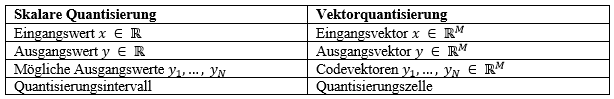
\includegraphics[width=1.0\textwidth]{img/Stephan.png}
	\caption[Quantisierungsverfahren]{Quantisierungsverfahren}
	\label{fig:stephan_quant}
\end{figure}

\subsection{\textbf{Anfordeungen für Inbetriebnahme und Einsatz}}

%\subsubsection{Sicherheitsziele}
%Der Benutzername und das Passwort werden in einem gesicherten Speicherbereich (nur root), mit \acs{AES} verschlüsselt, gespeichert.
%Die Datenbank in der die Noten gespeichert werden, liegt ebenfalls in diesem Bereich und darf nur von der \acs{HfTL}-App geöffnet werden.
%Die Kommunikation mit der \acs{HfTL}-Webseite und \acs{QIS} erfolgt gesichert per \acs{HTTPS}.



\subsubsection{Installationsprozedur}

Die \acs{APP} wird als .apk Datei ausgeliefert und kann somit manuel auf Android-Smartphones ab Version 4.4.2 installiert werden.
Dabei muss das Installieren von Software mit unbekannter Herkunft erlaubt werden.




\subsection{\textbf{Qualitätsanforderungen}}

\subsubsection{Qualitätsmerkmale}
Folgende Qualitätsansprüche werden gestellt:
\begin{itemize}
	\item Hohe Zuverlässigkeit der Software
	\item schnelle und zuverlässige Verarbeitung der gewünschten Daten
	\item Fehler werden mit einer entsprechenden Fehlermeldung beantwortet
	\item Intuitiv benutzbar
	\item Leicht zu warten und zu erweitern
	\item Vollständige Dokumentation des Projektes
\end{itemize}


\subsection{\textbf{Anforderung an die Entwicklung}}

\subsubsection{Entwicklungs-Umgebung}
Für die Entwicklung wird Android Studio inkl. Gradle in der Version 1.x genutzt. Für die Dokumentation und Projektkoordination wird GitHub verwendet.
Die Dokumentation wird mittels \LaTeX{} erstellt.



%\subsubsection{Projekt-Organisation}
%Die Projektorganisation wird wie in folgender Abbildung strukturiert. Als Vorgehensmodell wird das Spiralmodell mit Prototyping gewählt. Es ist ein iteratives Modell, wobei jeder Zyklus in den einzelnen Quadranten folgende Aktivitäten enthält:
%
%\begin{itemize}
%	\item Festlegung von Zielen, Identifikation von Alternativen und Beschreibung von Rahmenbedingungen
%	\item Evaluierung der Alternativen und das Erkennen, Abschätzen und Reduzieren von Risiken, z. B. durch Analysen, Simulationen oder Prototyping
%	\item Realisierung und Überprüfung des Zwischenprodukts
%	\item Planung des nächsten Zyklus der Projektfortsetzung.
%\end{itemize}
%
%Die einzelnen Aufgaben werden Personen zugeordnet. In wöchentlichen Online-Meetings über Teamviewer stellt jeder seine Ergebnisse vor und es werden diese bewertet. Anhand dieser Ergebnisse werden für den neuen Zyklus Aufgaben verteilt. Der Protokollführer hält alle Ergebnisse und Aufgaben fest und legt die Protokolle im Projektordner ab.
%
%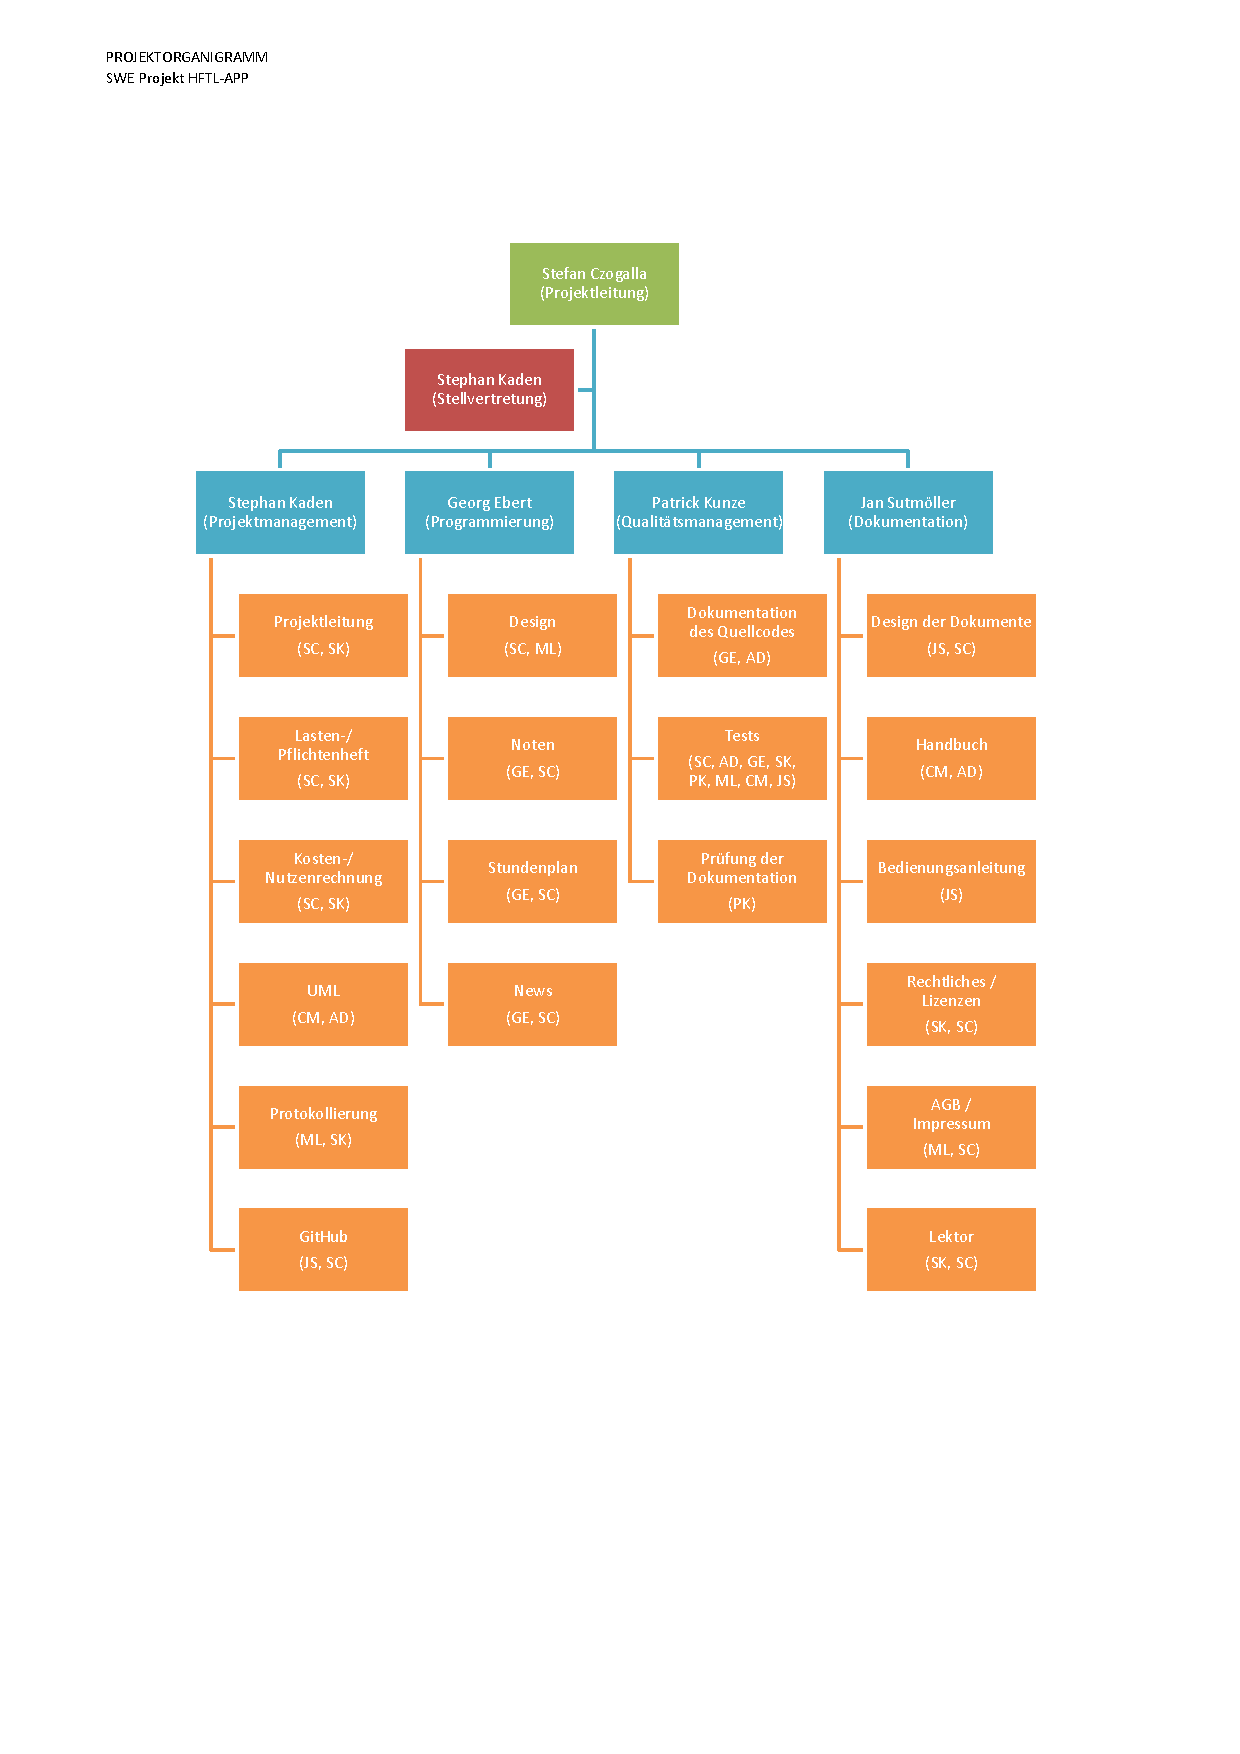
\includepdf[pages=-,noautoscale]{04_Anhang/files/swe_organigramm2.pdf}
%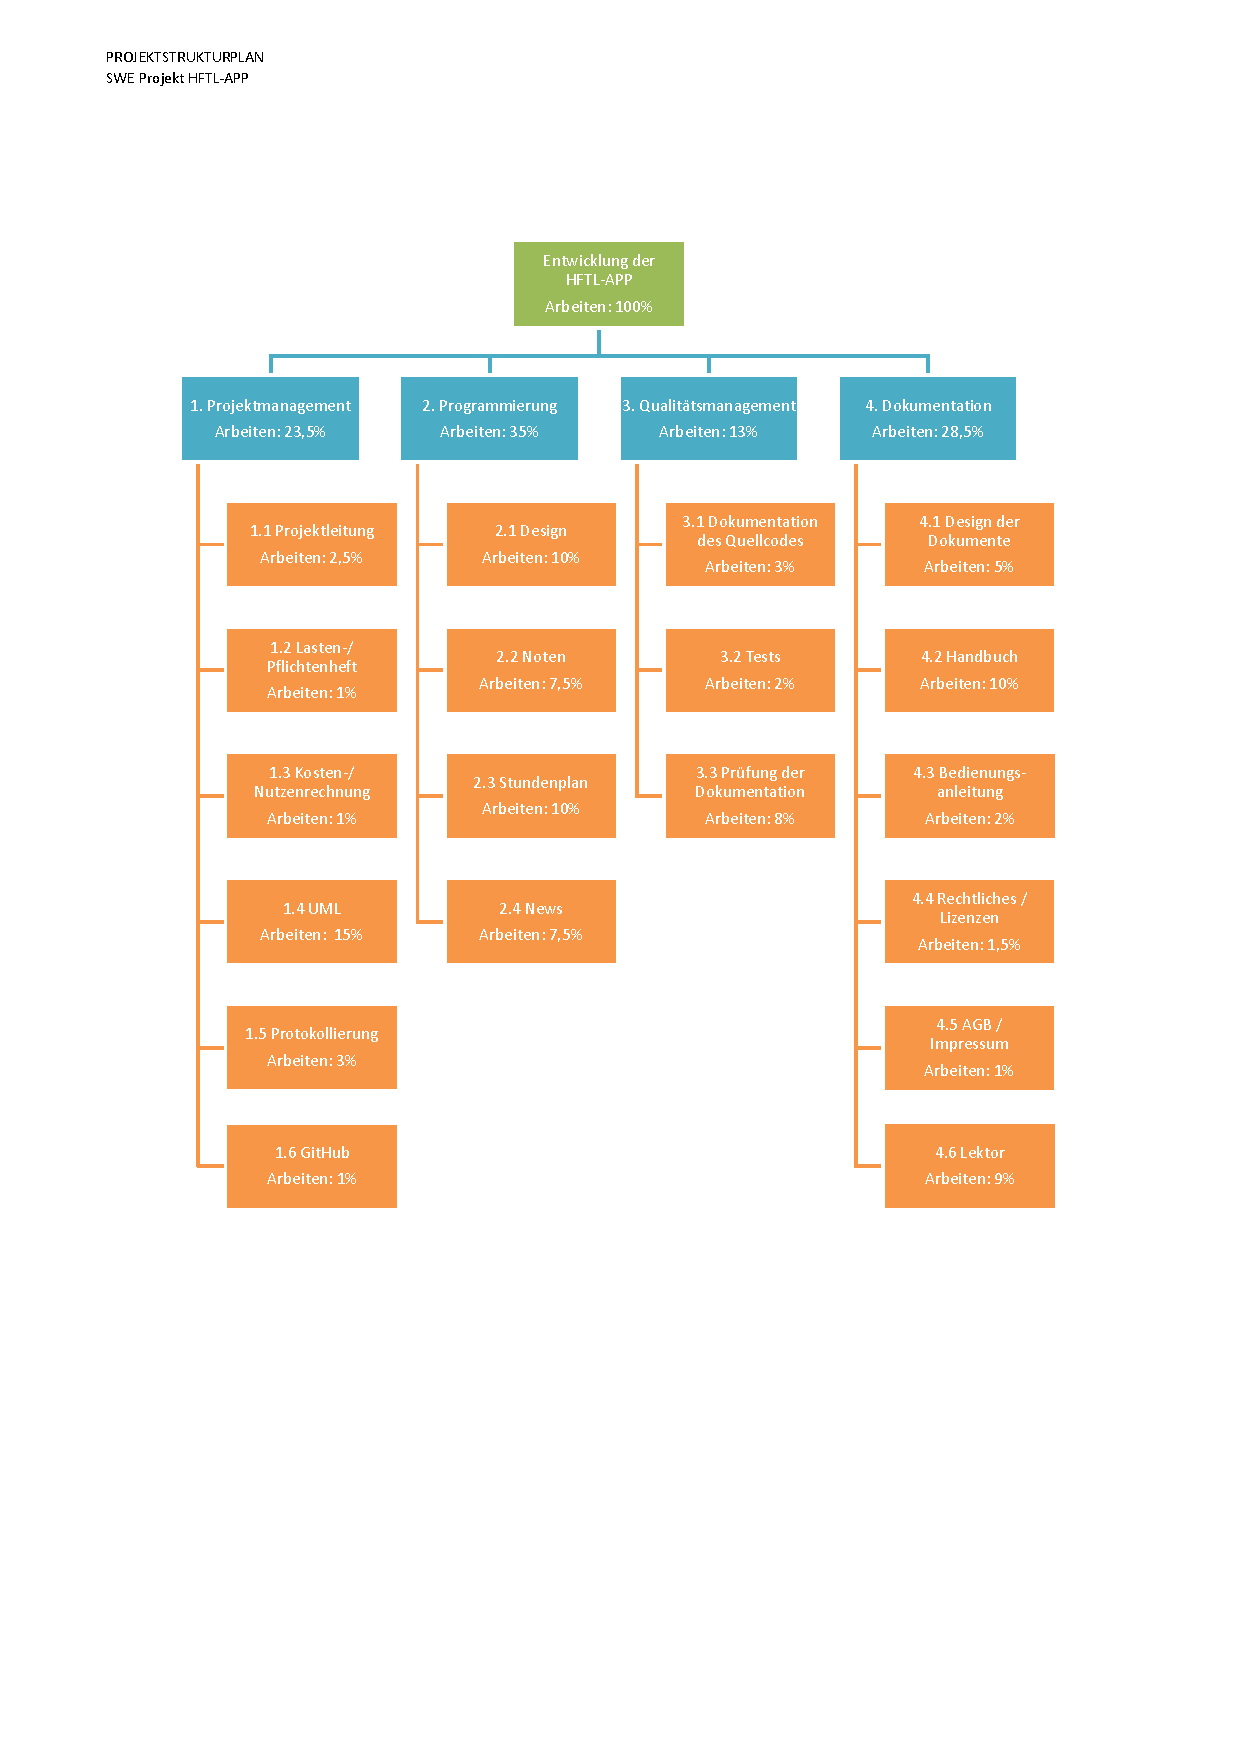
\includepdf[pages=-,noautoscale]{04_Anhang/files/swe_projektstrukturplan.pdf}


%\subsubsection{Projekt-Planung}
%siehe Anhang "'Gantt"' \ref{subsec:Gantt}

\subsubsection{Änderungsmanagement}
Zur Versionsverwaltung wurde Git eingesetzt. Als Hosting-Anbieter wurde dabei auf GitHub gesetzt, welcher einen kostenfreien Zugang für nicht kommerzielle Projekte bereitstellt. Ein \ac{GUI} oder ein Konsolenprogramm für Windows und Linux übernehmen dabei die Steuerung der Versionsverwaltung. Konflikte in den einzelnen Versionen können nur über die Konsole behoben werden. Auf der Webseite von GitHub können Milestones erstellt werden und an die jeweiligen Mitarbeiter zugeteilt werden. In den Milestones werden einzelne Aufgaben, sogenannte Issues angelegt und wiederum den Bearbeitern zugeordnet, somit ist der Bearbeitungsstand zu jeder Zeit des Projektes ersichtlich und es kann schnell auf sich ergebende Probleme reagiert werden.



%\subsubsection{Testanforderungen}
%siehe Anhang "'Testprotokollentwurf"' \ref{subsec:Testprotokollentwurf}

\section{Ergebnis}
\subsection{Umfang der APP}
Die App wurde, angelehnt an die Namen der vorhandenen Apps, "QuantiPig" genannt. Als Logo wurde ein Schweinekopf gewählt.
\begin{figure}[h]
	\centering
		
\includegraphics[width=0.4\textwidth]{img/ic_launcher.png}
	\caption[QuantiPig Logo]{QuantiPig Logo}
	\label{fig:pig_logo}
\end{figure}

Als Algorithmen wurde folgende Verfahren implementiert:

\begin{itemize}
	\item keine Quantisierung
	\item skalare Quantisierung mit folgenden Quantisierungsintervallen
		\begin{itemize}
			\item 2x2 px
			\item 4x4 px
			\item 8x8 px
			\item größtmögliche Quadrate (ggT)
		\end{itemize}
	\item Midtread-Quantisierung
\end{itemize}


\newpage
\subsection{Erscheinungsbild}
Die APP startet generell im Landscape-Modus. Wie in der folgenden Abbildung zu sehen, gibt es jeweils einen Button für die Wahl des Quantisierungsverfahrens und den Auslöser.

\begin{figure}[h]
	\centering
		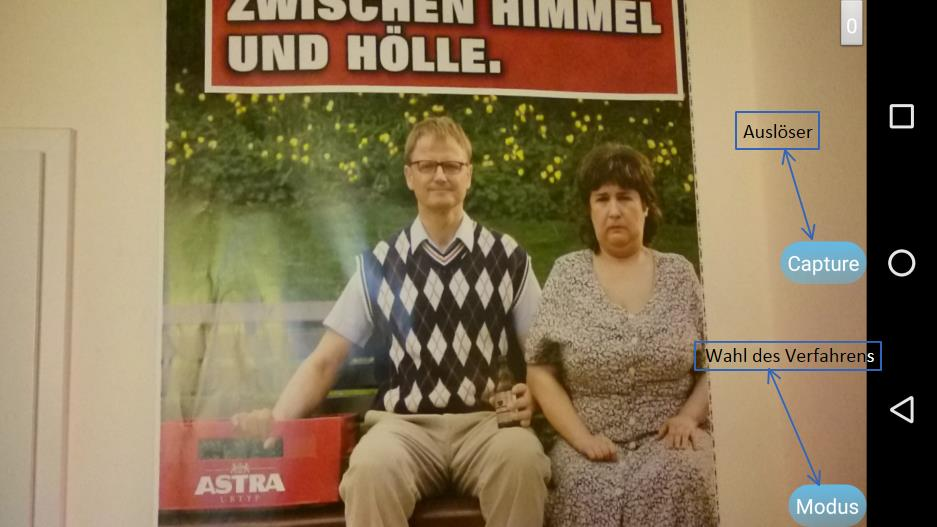
\includegraphics[width=1.0\textwidth]{img/Startbildschirm_QuantiPig.jpg}
	\caption[QuantiPig Startbildschirm]{QuantiPig Startbildschirm}
	\label{fig:pig_menue}
\end{figure}

Nach Drücken auf den Auslöser wird ein Foto mit aktuellem Komprimierungsverfahren gemacht und in den entsprechenden Ordner auf dem Smartphone abgelegt. Als Name wird das jeweilige Verfahren, gefolgt von einem Zeitstempel verwendet.

Nach betätigen des Buttons \glqq
Modus\grqq
, öffnet sich, wie in folgender Abbildung zu sehen, ein Auswahlmenü für die drei verschiedenen Verfahren.

\begin{figure}[h!]
	\centering
		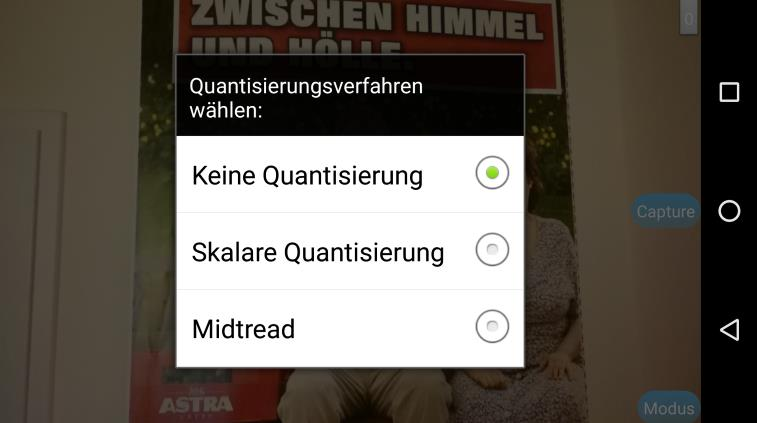
\includegraphics[width=1.0\textwidth]{img/Verfahren_QuantiPig.jpg}
	\caption[QuantiPig-Menü Verarbeitungsverfahren]{QuantiPig-Menü Verarbeitungsverfahren}
	\label{fig:pig_verfahren}
\end{figure}

Im Modus skalare Quantisierung gibt es einen weiteren Button mit dem man das Quantisierungsintervall auswählen kann.

\begin{figure}[h!]
	\centering
		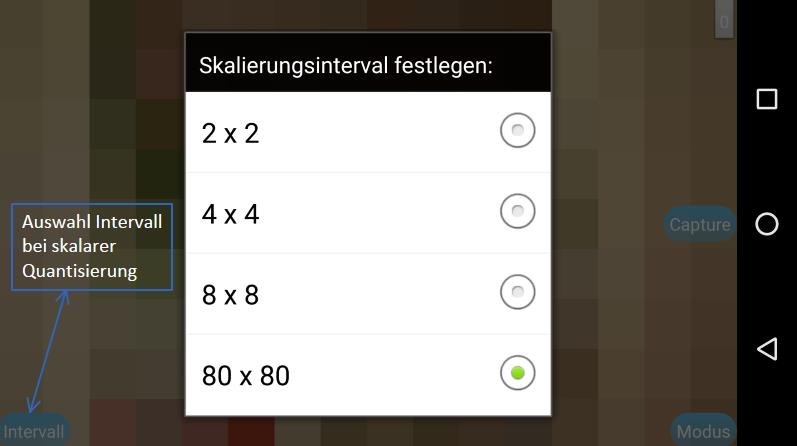
\includegraphics[width=1.0\textwidth]{img/Intervall_QuantiPig.jpg}
	\caption[QuantiPig-Menü Qunatisierungsintervall]{QuantiPig-Menü Qunatisierungsintervall}
	\label{fig:pig_intervall}
\end{figure}


\clearpage

\newpage
\subsection{Quellcode}
\subsubsection{Allgemein}

Der grundlegende Aufbau des Quellcodes wurde von der vorgegebenen App "'FotoQuuant"' übernommen. So wurden ebenfalls drei Klassen generiert:
\begin{itemize}
	\item MainActivity.java
	\item CameraView.java
	\item CameraListener.java
\end{itemize}
Im Folgenden wird nicht auf jedes Detail im Quellcode eingegangen, jedoch die wichtigsten Funktionen erläutert.

\subsubsection{MainActivity.java}
\label{mainactivity}

Die MainActivity ist die Haupt- und damit Startaktivität der App. Hauptaufgabe der Aktivität ist es, Objekte  (Strings, Buttons, Menüs, Ladebalken etc.) beim Start der App aufzurufen und ggf. mit Aktions-Listener zu versehen, sofern die Objekte hier auf Nutzereingaben reagieren sollen. \\
Dies geschieht innerhalb der Methode "'\textit{onCreate();}"', die das Layout einer View zuordnet und anschließend bereits erwähnte Objekte instanziert. \\
\\
Folgender Ausschnitt zeigt am Beispiel von mCameraView, wie dieses einem Layoutobjekt (\textcolor{lila}{\textit{suface\_view}})  zugeordnet wird, die Sichtbarkeit manipuliert wird und mit dem \hyperref[CameraListener]{CameraListener}  bestückt wird:

\lstset{language = JAVA}

\begin{lstlisting}
	setContentView(R.layout.activity_main);
		
	mCameraView = (CameraView) findViewById(R.id.surface_view);
	mCameraView.setVisibility(SurfaceView.VISIBLE);
	mCameraView.setCvCameraViewListener(new CameraListener());
\end{lstlisting}

Darüber hinaus sind hier einige wichtige Methoden aufgeführt, die essentiell für die Funktionsweise von OpenCV und somit für die App als funktionierende Smartphone-Kamera sind:
\begin{itemize}
\item onResume()
\item BaseLoaderCallback (hier wird die Klasse \hyperref[CameraView]{CameraView}) aufgerufen)
\item onPause()
\item onDestroy();
\item onStart();
\end{itemize}
Weitere Details können auch der \href{http://docs.opencv.org/2.4/doc/tutorials/introduction/android_binary_package/dev_with_OCV_on_Android.html#dev-with-ocv-on-android}{OpenCV-Dokumentation} entnommen werden.


\subsubsection{CameraView.java}
\label{CameraView}

Dies ist das funktionale Kernstück der App. Hier werden die Bildbearbeitungsalgorithmen auf das Live-Bild und auf das zu speichernde Bild gelegt. 
\\
\begin{description}
\item[quantiMode0 - Original]~\par
\label{quantimode0}
Dieser Modus ist der Standardmodus beim Starten der App und kann als Standardrahmen für die anderen Modi gesehen werden.\\ 
Diese Methode dient als reiner Durchlauf und soll lediglich sicherstellen, dass das \textit{unbearbeitete} Bild genauso behandelt wird, wie die \textit{bearbeiteten} Bilder. Der Methode wird das Bild als Array mitsamt Höhe und Breite übergeben und die Methode gibt das Array unbehandelt wieder zurück. 
\begin{lstlisting}
    public static byte[] quantiMode0(byte[] buff, int mHeight, int mWidth) {
        return buff;
    }
\end{lstlisting}

\item[quantiMode1 - Skalar]~\par
\label{quantimode1}
Dieser Modus ist der aufwändigste. Allgemein wird nichts anderes gemacht, als die RGBA-Werte der Bildpunkte innerhalb eines Quadrates (die Kantenlänge entspricht dem \hyperref[intervall]{Intervall}) in ein neues Array (kanalweise) addiert. Der Index dieses neuen Arrays entspricht dabei dem abgetasteten Intervallquadrat. Sobald dies mit dem kompletten Bild geschehen ist, wird der Durchschnitt aus diesen RGBA-Werten (kanalweise) errechnet und wieder zurück in das originale Array übergeben. Somit entsteht - je nach Größe des Intervalls - ein immer mehr grobkörniges Bild.\\ 
\\\
Die erste Besonderheit dieses Algorithmus ist, dass dieser nicht direkt durch Auswahl im Menü aufgerufen wird, sondern über den Umweg über die Methode \hyperref[interval]{setCluster()}. Dies führt zur zweiten Besonderheit: Diese Methode bekommt neben dem Array und den Werten für Breite und Höhe des Bildes zusätzlich noch das Intervall (\textit{cluster}) als Parameter übergeben.
\begin{lstlisting}
public static byte[] quantiMode1(byte[] buff, int mHeight, int mWidth, int cluster){ 
	...
	return buff;
} 
\end{lstlisting}

Zunächst werden einige Variablen mit \textcolor{blau}{0} instanziert.
\begin{lstlisting}
        int x = 0;
        int k = 0;                                                                                  
        int countY = 0;                                                                             
        int[] frame = new int[mWidth / cluster * mHeight / cluster * 4];                            
\end{lstlisting}
Kurze Eräuterung:
\begin{itemize}
\item x: Index des abzutastenden Farbwertes auf buff
\item k: Index des RGBA-Bildpunktes des Hilfsarrays frame
\item countY: Zähler, wie viele Zeilen von buff schon abgetastet wurden
\item frame: Das Hifsarray zur Berechnung des Durchschnitts.   
\end{itemize}
Nun beginnt das Abtasten und das Überschreiben der Werte aus buff in frame mit Hilfe von vier ineinander verschachtelten Schleifen.\\
Die äußere Schleife geht vertikal, also zeilenweise das Bild runter:
\begin{lstlisting}
         for (int n = 0; n < mHeight; n++) {                                                         
\end{lstlisting}
Es ist notwendig die Anzahl abgetasteten Zeilen zu kennen. Daher wird jeder Schleifendurchlauf der äußeren Schleife mitgezählt.
\begin{lstlisting}
            countY++;                                                                               
\end{lstlisting}
Nun beginnt der Schleifendurchlauf in der Horizontalen. Als erstes wird jedes Cluster einzeln durchlaufen.
\begin{lstlisting}
            for (int m = 0; m < mWidth / cluster; m++) {                                            
\end{lstlisting}
Danach wird jeder Bildpunkt im Cluster durchlaufen.
\begin{lstlisting}            
                for (int j = 0; j < cluster; j++) {                                                 
\end{lstlisting}
Und nun werden die RGBA-Kanäle des Bildpunktes durchlaufen. 
\begin{lstlisting}
                    for (int i = 0; i < 4; i++) {                                                   
\end{lstlisting}
Zusammenfassung:
\begin{itemize}
\item x = Index des Quell-Arrays
\item k = Index des Ziel-Arrays
\item n = Zeile des Quell-Arrays
\item m = Index des Clusters in der Zeile
\item j = Index des Bildpunktes innerhalb des Clusters
\item i = Index des RGBA-Kanals im Bildpunkt   
\end{itemize}
Damit können nun alle Koordinaten durchlaufen werden. Die Sache wird nur noch dadurch komplizierter, da JAVA mit signed-Werten arbeitet und sich somit der Wert inhaltlich ändert. (Wertebereich ändert sich von (0 bis 255) auf (-128 bis 127))\\
Daraus folgend werden Additionen mit Werten > 127 als Subtraktion ausgeführt. Dies wird vor allem dann an Kanten sichtbar, wo stark unterschiedliche Werte dicht beieinander liegen. Dieser Effekt wird ggf durch ein großes Intervall verstärkt. 
\\
(s. linkes Bild von \ref{fig:signedunsigned})

\begin{figure}[h]
	\centering
		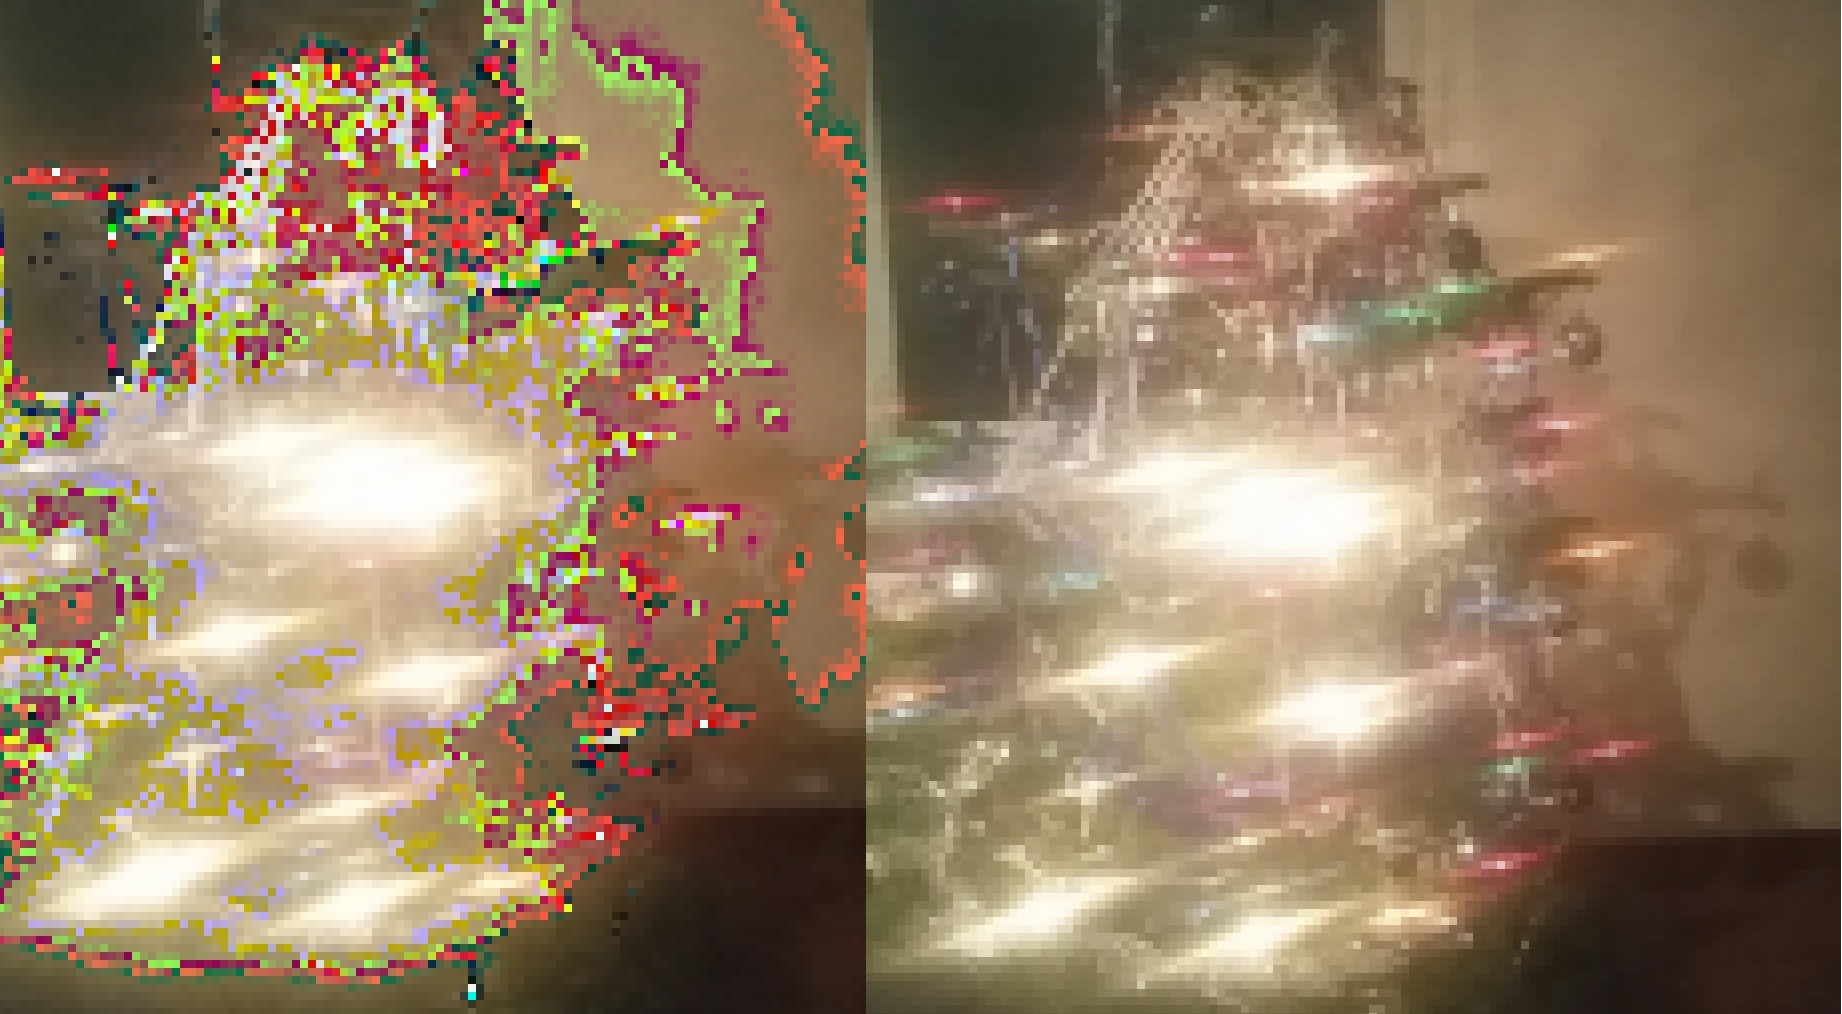
\includegraphics[width=1.0\textwidth]{img/signedUnsigned.jpg}
	\caption[signedunsigned]{Gleiches Motiv mit einem 8 x 8 Intervall aufgenommen}
	\label{fig:signedunsigned}
\end{figure}
Um das Problem zu umgehen und das Resultat wie im rechten Teil des Bildes zu erzielen, werden die negativen Werte umgerechnet.
\begin{lstlisting}                    
                        if (buff[x + i + j * 4] >= 0)                                               
                            frame[k + i] += ((int) buff[x + i + j * 4]);                            
                        else
                            frame[k + i] += ((int) buff[x + i + j * 4] & 0xff);                     
                    }
                }
\end{lstlisting}
Mit dem Schließen der inneren beiden Schleifen wurde das erste Cluster (m=0) in der ersten Zeile vollständig abgetastet der erste Bildpunkt des Hilfsarray (zunächst) fertig befüllt. Daher wird wird der Index des Zielarrays um einen Bildpunkt, also um 4 (aufgrund der vier Kanäle) erhöht. Gleichzeitig springt der Index des Quell-Arrays auf den ersten Bildpunkt der in das neue Cluster geschrieben werden soll. Dies wird so lange gemacht, bis das Zeilenende erreicht wurde.
\begin{lstlisting}                 
                k += 4;                                                                             
                x += 4 * cluster;                                                                   
            }
\end{lstlisting}
Dies wird nun Zeile für Zeile so oft wiederholt. Da der Algorithmus auch Bildpunkte eines Cluster abtasten muss, die untereinander liegen, muss nach jedem Zeilendurchlauf geprüft werden, ob die Clusterbreite (/-höhe) bereits erreicht wurde. Ist dies nicht geschehen, werden alle untereinander stehenden Werte in den selben Index des Ziel-Arrays geschrieben, womit dieser immer wieder am Zeilenanfang zurückgesetzt werden muss.
\begin{lstlisting}            
            if (countY < cluster)                                                                   
                k -= mWidth * 4 / cluster;                                                          
\end{lstlisting}
Wurden nun auch in der Vertikalen alle Bildpunkte abgetastet, dürfen sich alle Indexe erhöhen. Nur das Zählen der Schleifendurchläufe, bis wieder die Clusterhöhe erreicht wurde, muss von vorne beginnen.
\begin{lstlisting}
            else
                countY = 0;                                                                         
        }
\end{lstlisting}
Nach dem nun alle Werte in das cluster-weise übertragen und im Hilfsarray aufsummiert wurden, muss nur noch der Durchschnitt berechnet werden (Summe der Elemente : Anzahl der Elemente). Bei der Methode muss man sich jedoch im Klaren sein, dass hier aufgrund des verwendeten Datentyps \textcolor{darkblue}{integer} eine Ganzzahldivision stattfindet, was am Ende zu Rundungsfehlern führt.
\begin{lstlisting}
        for (int i = 0; i < frame.length; i++) {
                    frame[i] = frame[i] / (cluster * cluster);
        }
\end{lstlisting}
Nun werden die Durchschnittswerte wieder zurück in das Quell-Array geschrieben. Dabei werden die gleichen vier Schleifen wie zuvor durchlaufen. 
\begin{lstlisting}
        k = 0;
        countY = 0;
        x = 0;

        for (int n = 0; n < mHeight; n++) {
            countY++;

            for (int m = 0; m < mWidth / cluster; m++) {
                for (int j = 0; j < cluster; j++) {
                    for (int i = 0; i < 4; i++) {
                        buff[x + i + j * 4] = (byte) frame[k + i];
                    }
                }
                k += 4;
                x += 4 * cluster;
            }
            if (countY < cluster)
                k -= mWidth * 4 / cluster;
            else
                countY = 0;
        }
\end{lstlisting}


\item[quantiMode2 - Midtread]~\par
\label{quantimode2}

Dieser Modus wurde aus der App FotoQuant übernommen und optimiert. \\
Dabei wird der jeweilige Kanalwert bitweise um 5 Stellen nach rechts verschoben, sodass die 5 niederwertigsten Bits  aus dem Array entfernt werden. 
Die 5 höchstwertigen Bit werden - je nach Vorzeichen des Wertes mit 1 (bei negativen Werten) oder 0 (bei positiven Werten) aufgefüllt. 
\\
Anschließend wird der Inhalt des Arrays wieder bitweise um 5 Stellen nach links verschoben. Somit werden die 5 niederwertigsten Bit auf 0 gesetzt.
\\
\begin{lstlisting}
buff[t + j] = (byte) ((buff[t + j] >> 5) << 5);
\end{lstlisting}

Dadurch verringert sich der Farbraum von 16777216 (256 x 256 x 256) auf 512 (8 x 8 x 8) Farben. \textit{(Der Alphakanal wurde in der Berechnung nicht berücksichtigt.)} \\
Die Optimierung des Algorithmus bestand zum Einen aus der Entfernung einer if-Abfrage, ob die Werte im Arrays größer oder kleiner als 0 sind und zum Anderen werden alle Bildpunkte des Live-Bildes abgetastet und bearbeitet (vgl. \hyperref[fig:quant_mid]{Midtread(FotoQuant)} 


\item[setCluster]~\par
\label{intervall}
Folgende Intervalle sind implementiert:
\begin{itemize}
\item 2 x 2 (Standard)
\item 4 x 4 
\item 8 x 8
\item (Max) x (Max)
\end{itemize}
Im \textbf{Modus 8 x 8} müsste grundlegend eine Prüfung stattfinden, ob das Display restlos in Quadrate der Größe 8 aufteilbar ist, da sonst der Algorithmus in eine OutOfBoundsException läuft und die App anschließend abstürzt. Da dies jedoch nicht für die \textit{gängigen} Auflösungen zutrifft, wurde auf diese Sicherheitsmaßnahme der Einfachheit halber verzichtet. \\
\\\
\label{max}
Der letzte Modus kann als eine experimentelle Spielerei angesehen werden. Hier wird über die Methode \hyperref[ggt]{ggT} die maximale Intervallbreite des Displays ermittelt und angewandt. So werden bei einer Auflösung von 1920 x 1080 ein Bild von 16 x 9 Quadraten mit der Kantenlänge von 120 Bildpunkten angezeigt.\\



\item[ggT]~\par
\label{ggt}
Die Methode errechnet aus den übergebenen Werten (Höhe und Breite des Bildes) den größten gemeinsamen Teiler nach dem Euklidischen Algorithmus und übergibt diese an das \hyperref[max]{letzte Intervall} im \hyperref[quantimode1]{Skalar-Modus}.
\begin{lstlisting}
    private static int ggT(int zahl1, int zahl2){
        while (zahl2 != 0) {
            if (zahl1 > zahl2) {
                zahl1 = zahl1 - zahl2;
            } 
            else {
                zahl2 = zahl2 - zahl1;
            }
        }
        return zahl1;
    }
\end{lstlisting}

\subsubsection{CameraListener.java}
\label{CameraListener}
Diese Klasse nutzt als Interface die OpenCV-Klasse

 "'\textit{CameraBridgeViewBase.CvCameraViewListener2}"' 

Die Methode "'\textit{onCameraFrame()}"' erhält Einzelbilder von der Kamera und übergibt dieses an die Open-CV Klasse "'\textit{Mat}"' als RGBA-Matrix, welches wiederum von der Methode übergeben wird.

\begin{lstlisting}
   public Mat onCameraFrame(CameraBridgeViewBase.CvCameraViewFrame inputFrame) {
        Mat mRgba = inputFrame.rgba();
        return mRgba;
    }
\end{lstlisting}

s. hierzu OpenCV-Dokumentation:
\begin{itemize}
\item \href{http://docs.opencv.org/java/2.4.9/org/opencv/android/CameraBridgeViewBase.CvCameraViewListener2.html}{CvCameraViewListener2}
\item \href{http://docs.opencv.org/java/2.4.9/org/opencv/android/CameraBridgeViewBase.CvCameraViewFrame.html}{CvCameraViewFrame}
\end{itemize}

\end{description}






\subsection{Beispielbilder}
\begin{landscape}


\begin{figure}[h]
	\centering
		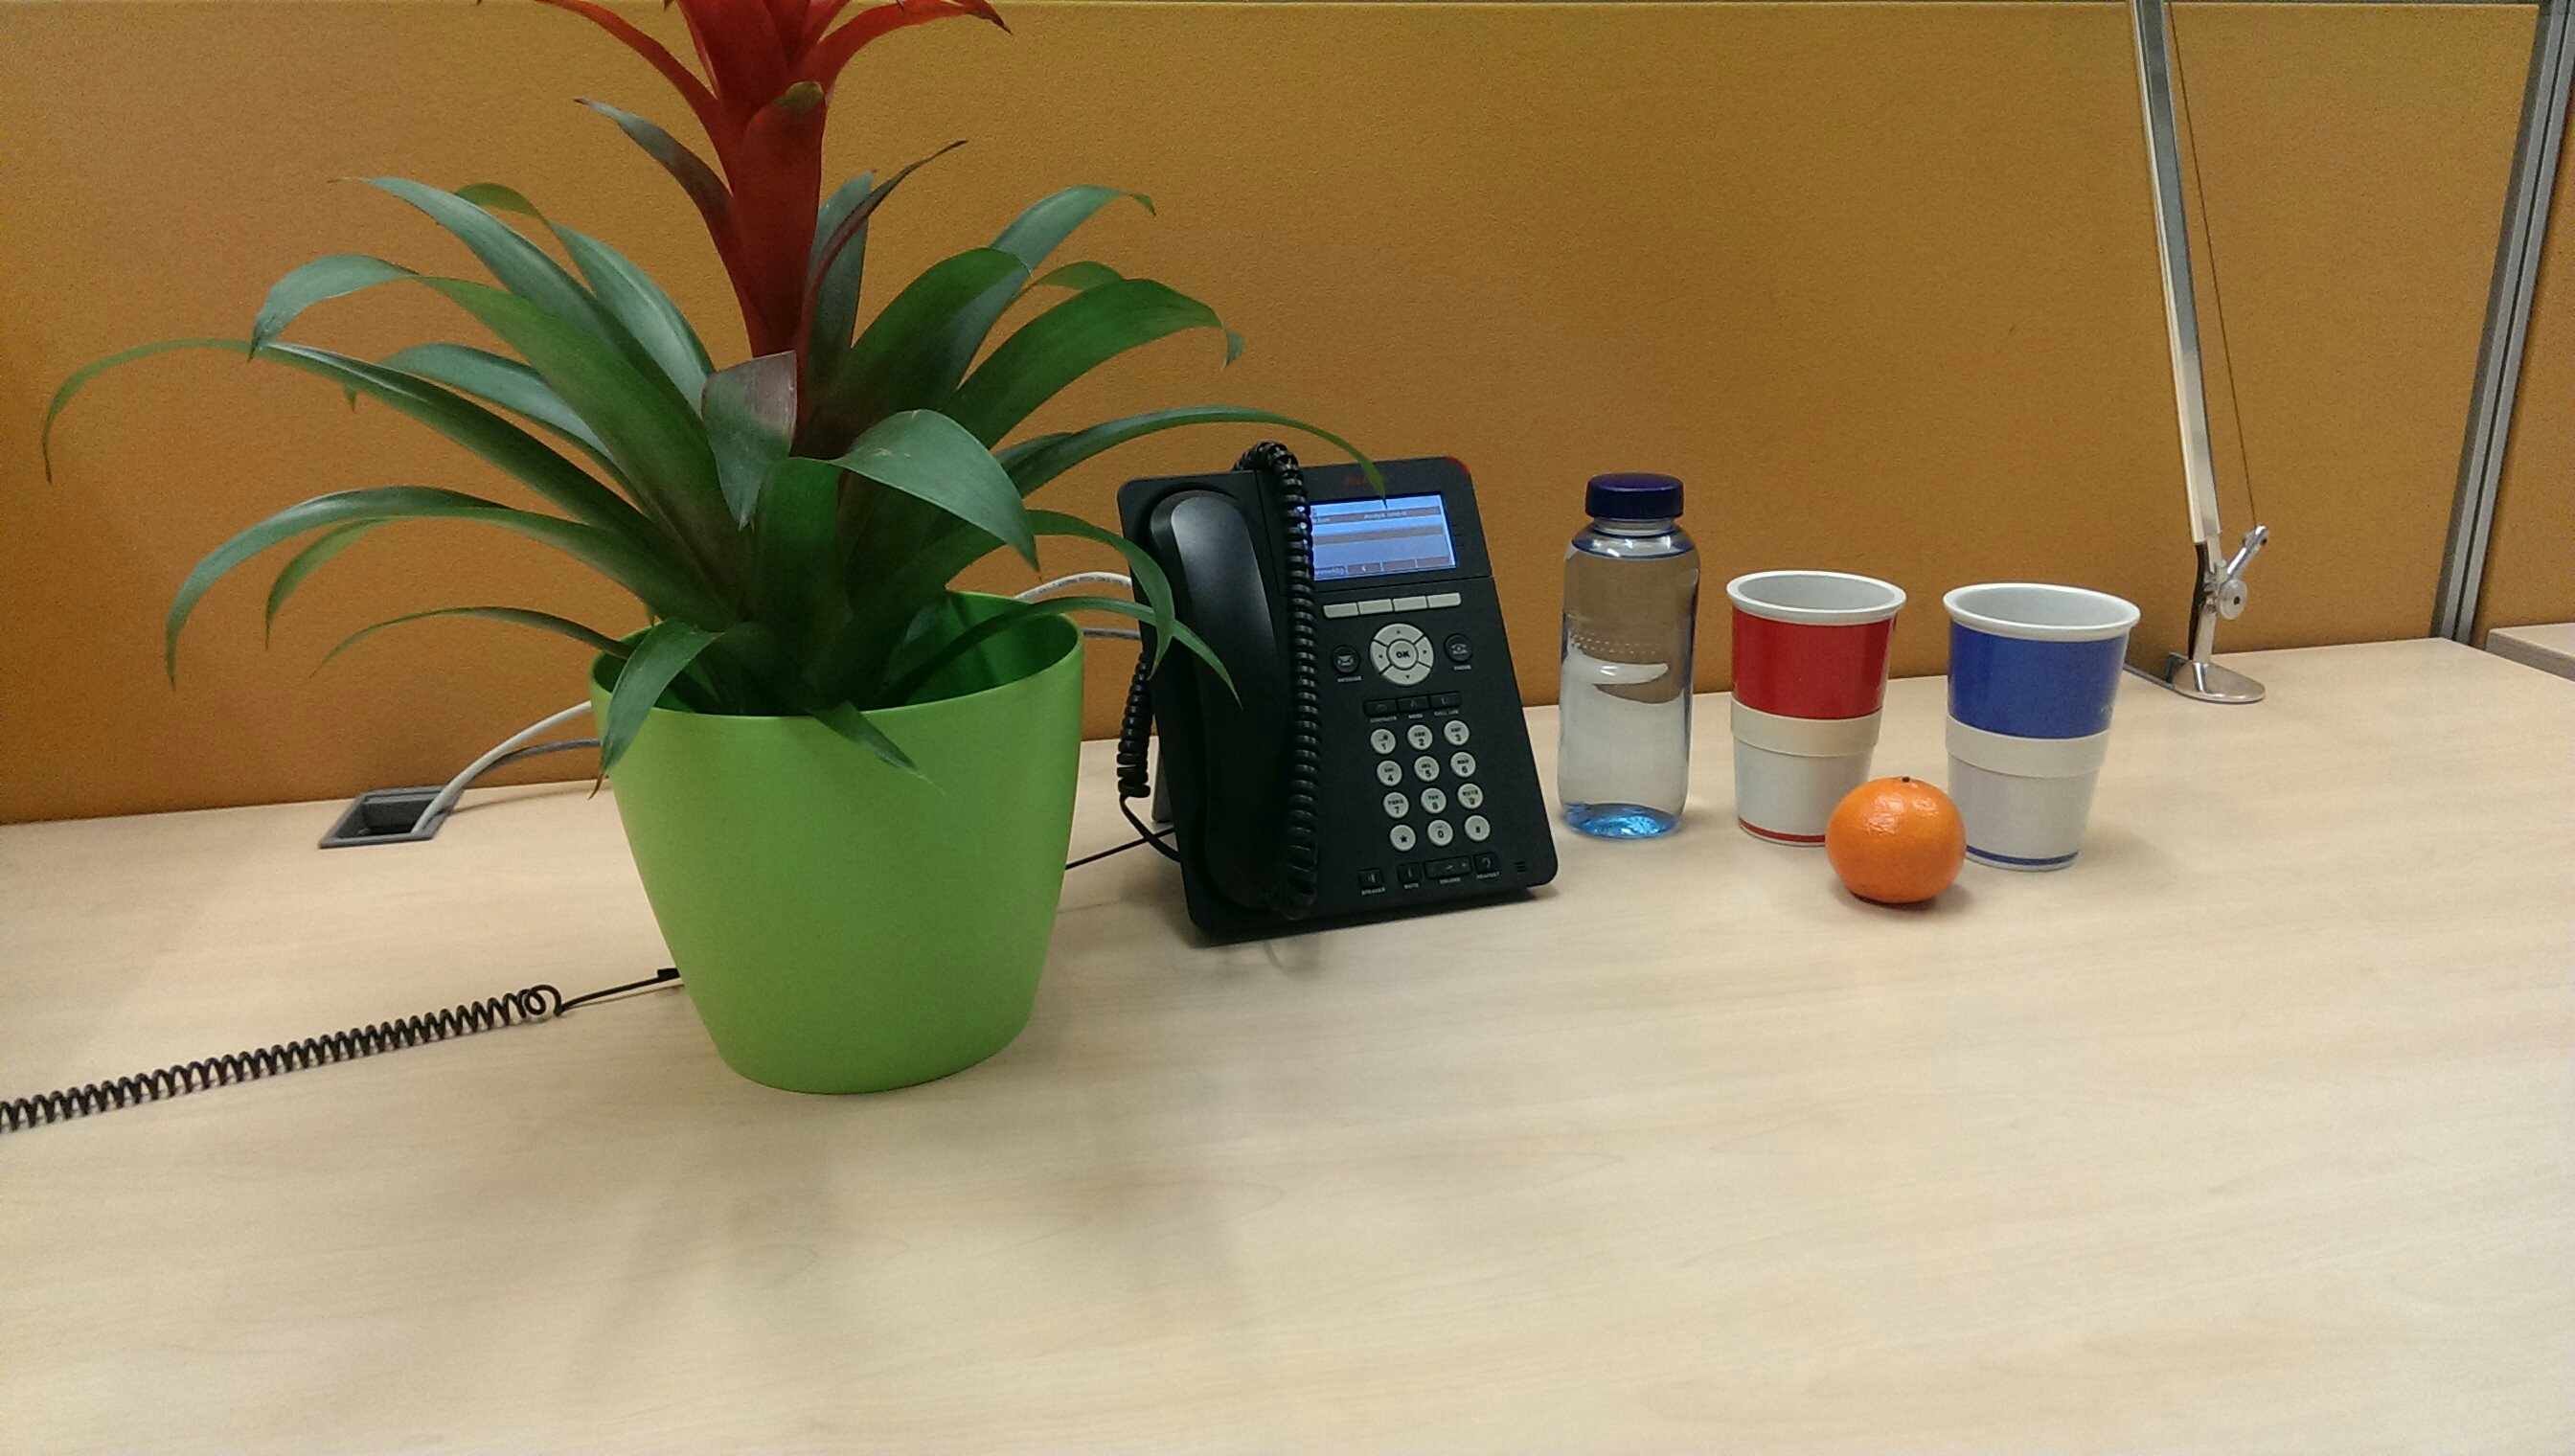
\includegraphics[width=1.4\textwidth]{img/Fotos/QuantiPig_Original.jpg}
	\caption[QuantiPig Originalbild]{QuantiPig Originalbild}
	\label{fig:pig_original}
\end{figure}

\begin{figure}[h]
	\centering
		\includegraphics[width=1.4\textwidth]{img/Fotos/QuantiPig_Midtread.jpg}
	\caption[QuantiPig Midtread]{QuantiPig Midtread}
	\label{fig:pig_midtread}
\end{figure}

\begin{figure}[h]
	\centering
		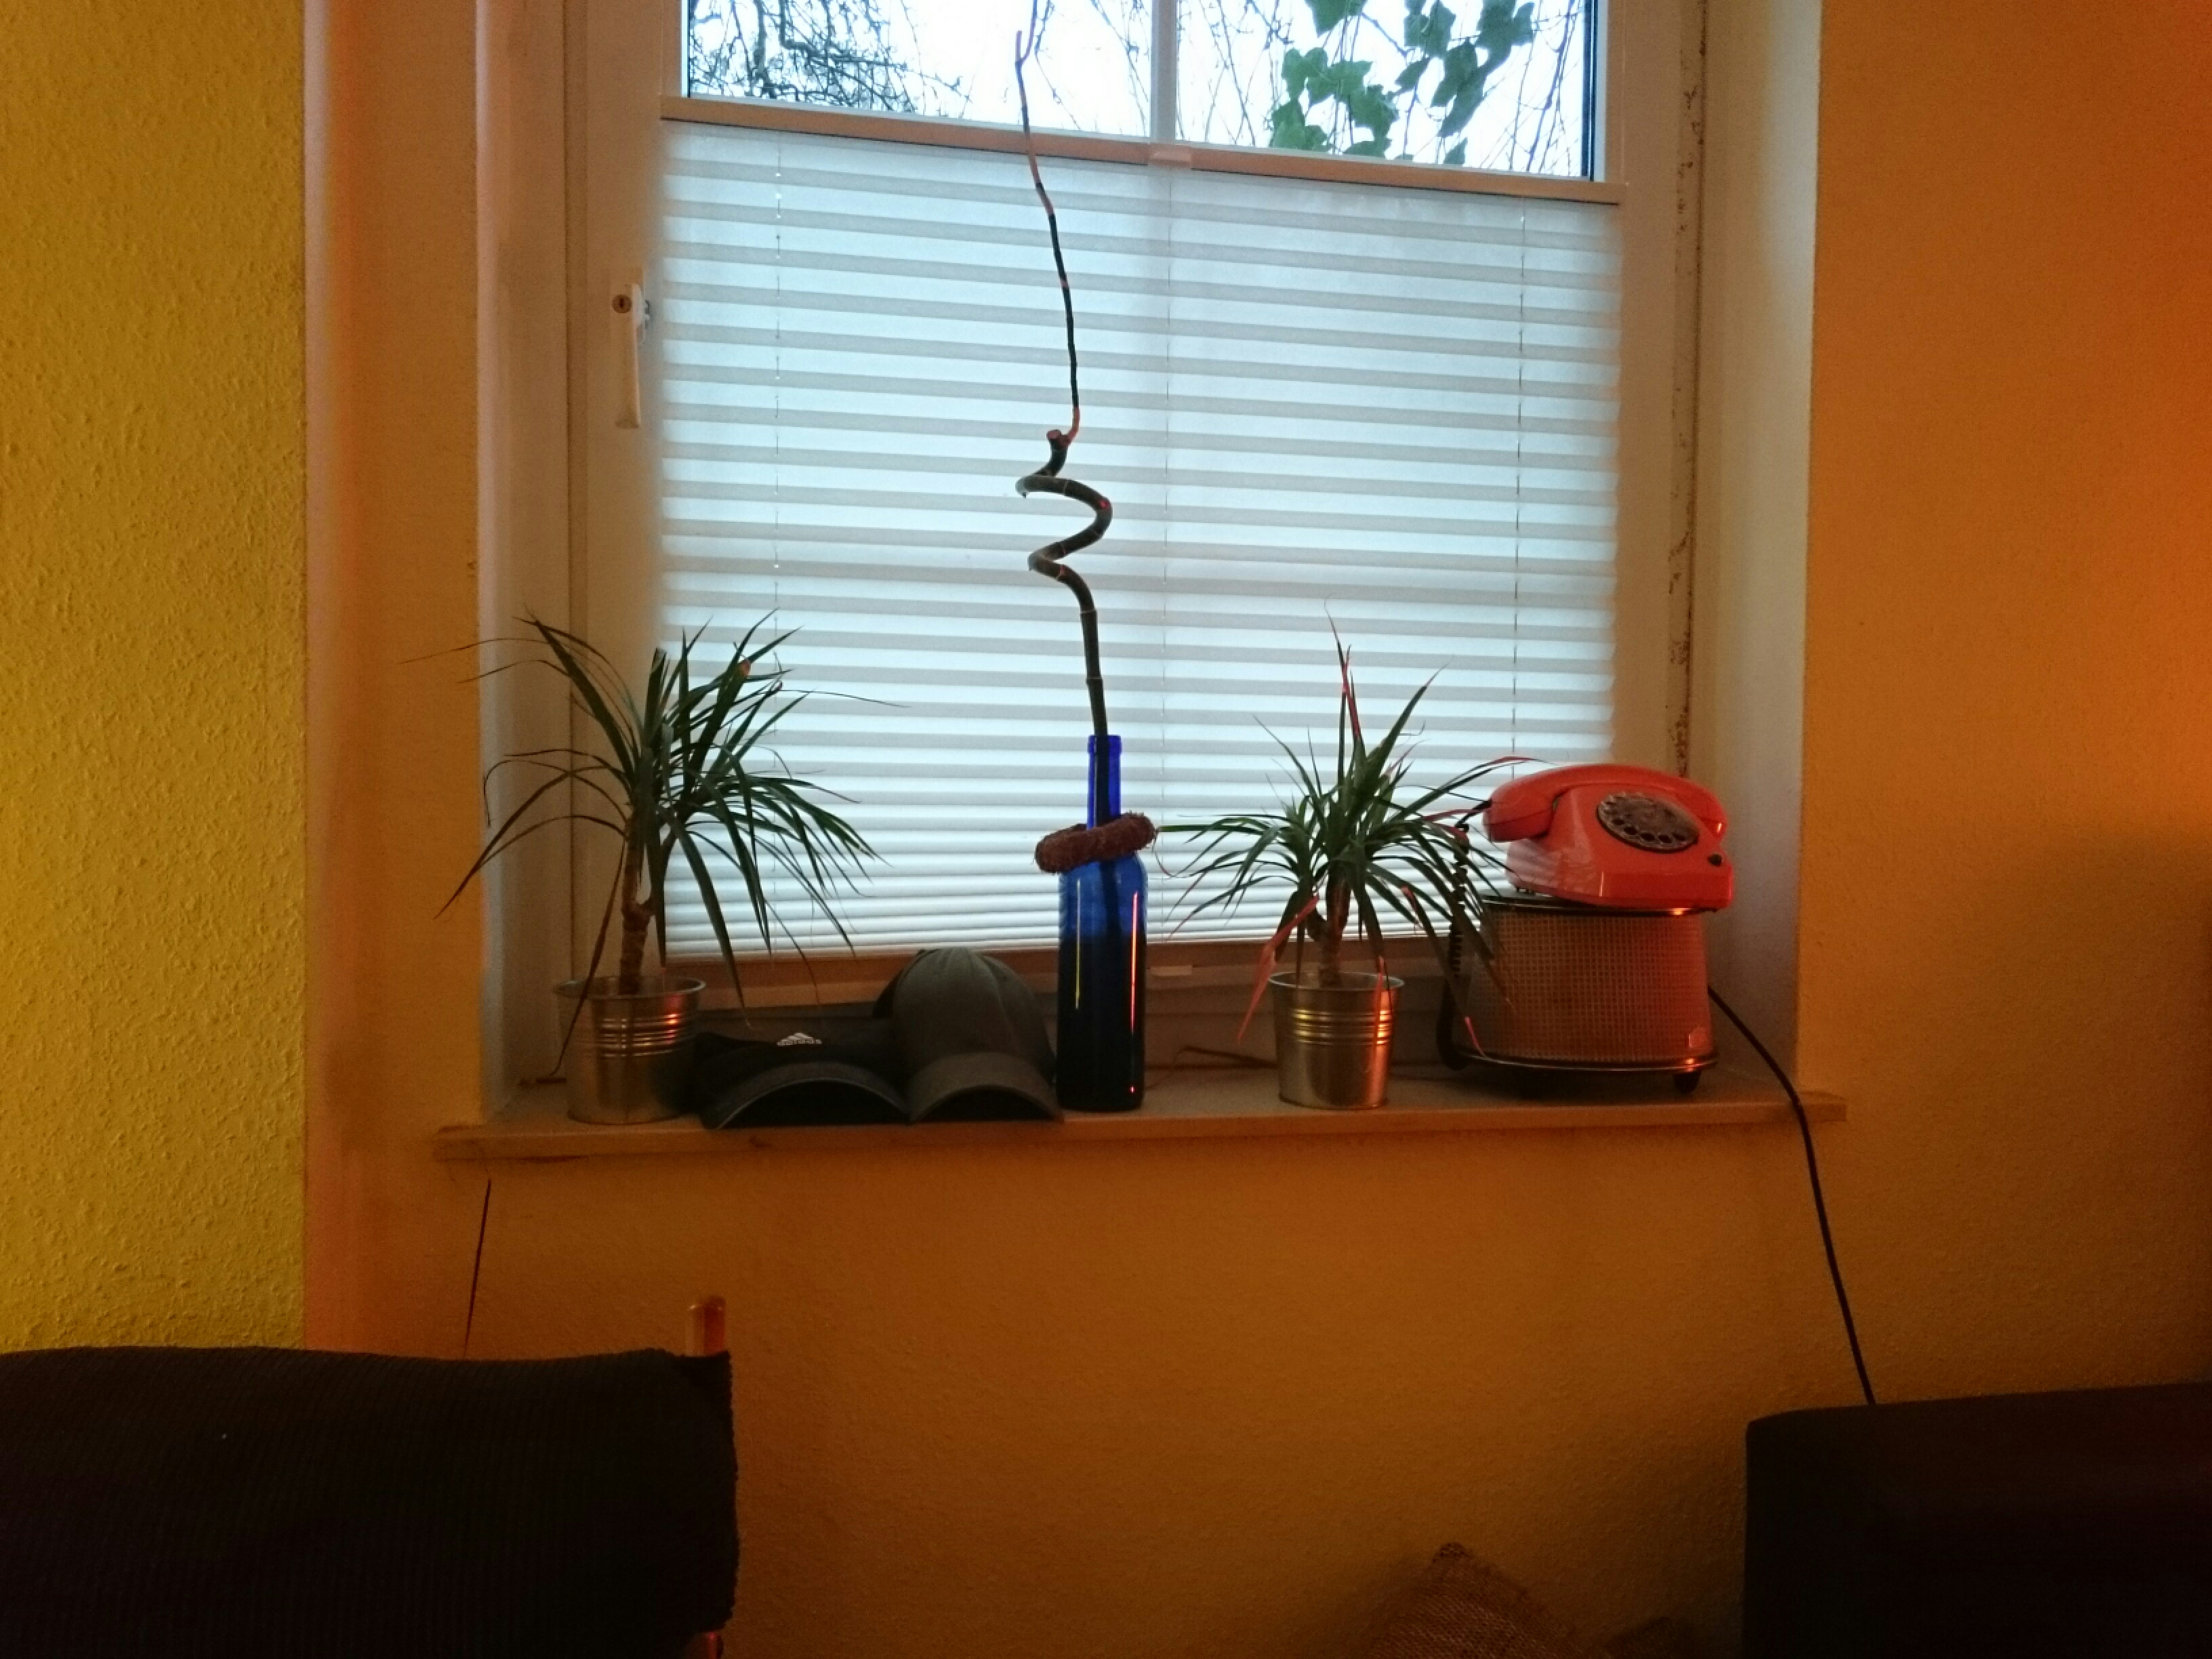
\includegraphics[width=1.4\textwidth]{img/Fotos/QuantiPig_Skalar_2x2.jpg}
	\caption[QuantiPig skalare Quantisierung 2x2 p]{QuantiPig skalare Quantisierung 2x2 px}
	\label{fig:pig_skalar 2x2}
\end{figure}

\begin{figure}[h]
	\centering
		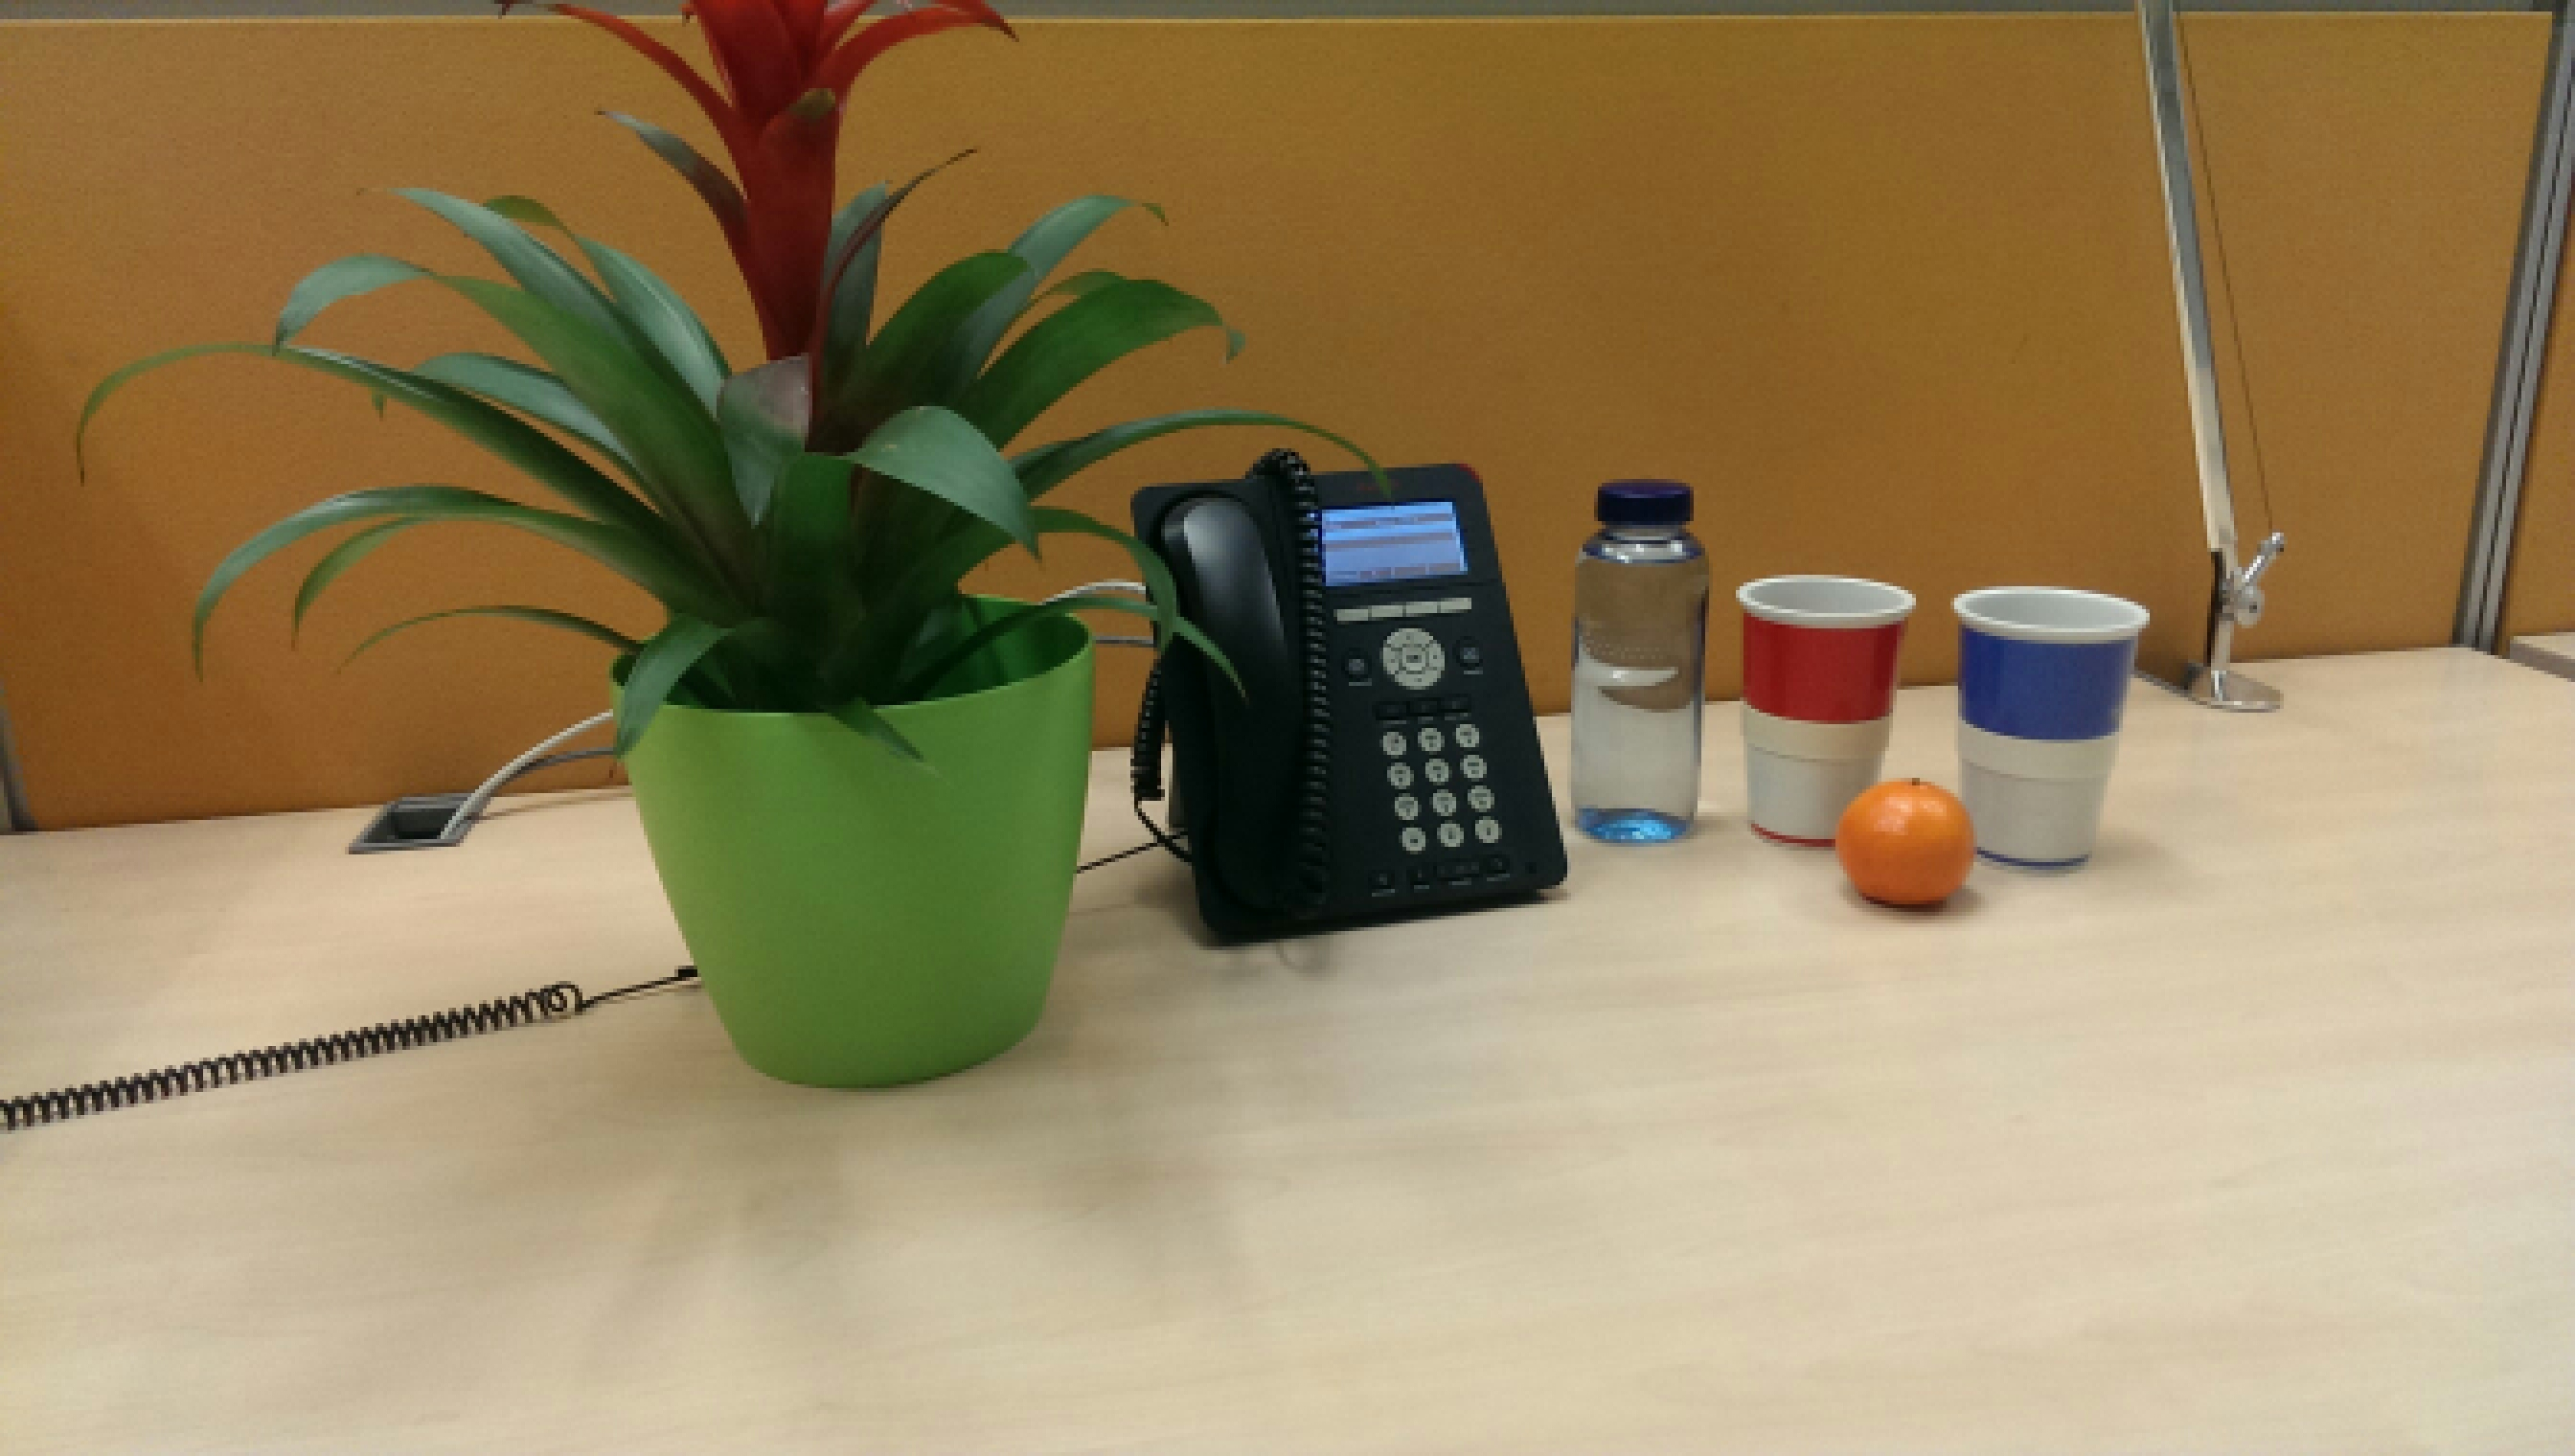
\includegraphics[width=1.4\textwidth]{img/Fotos/QuantiPig_Skalar_4x4.jpg}
	\caption[QuantiPig skalare Quantisierung 4x4 px]{QuantiPig skalare Quantisierung 4x4 px}
	\label{fig:pig_skalar 4x4}
\end{figure}

\begin{figure}[h]
	\centering
		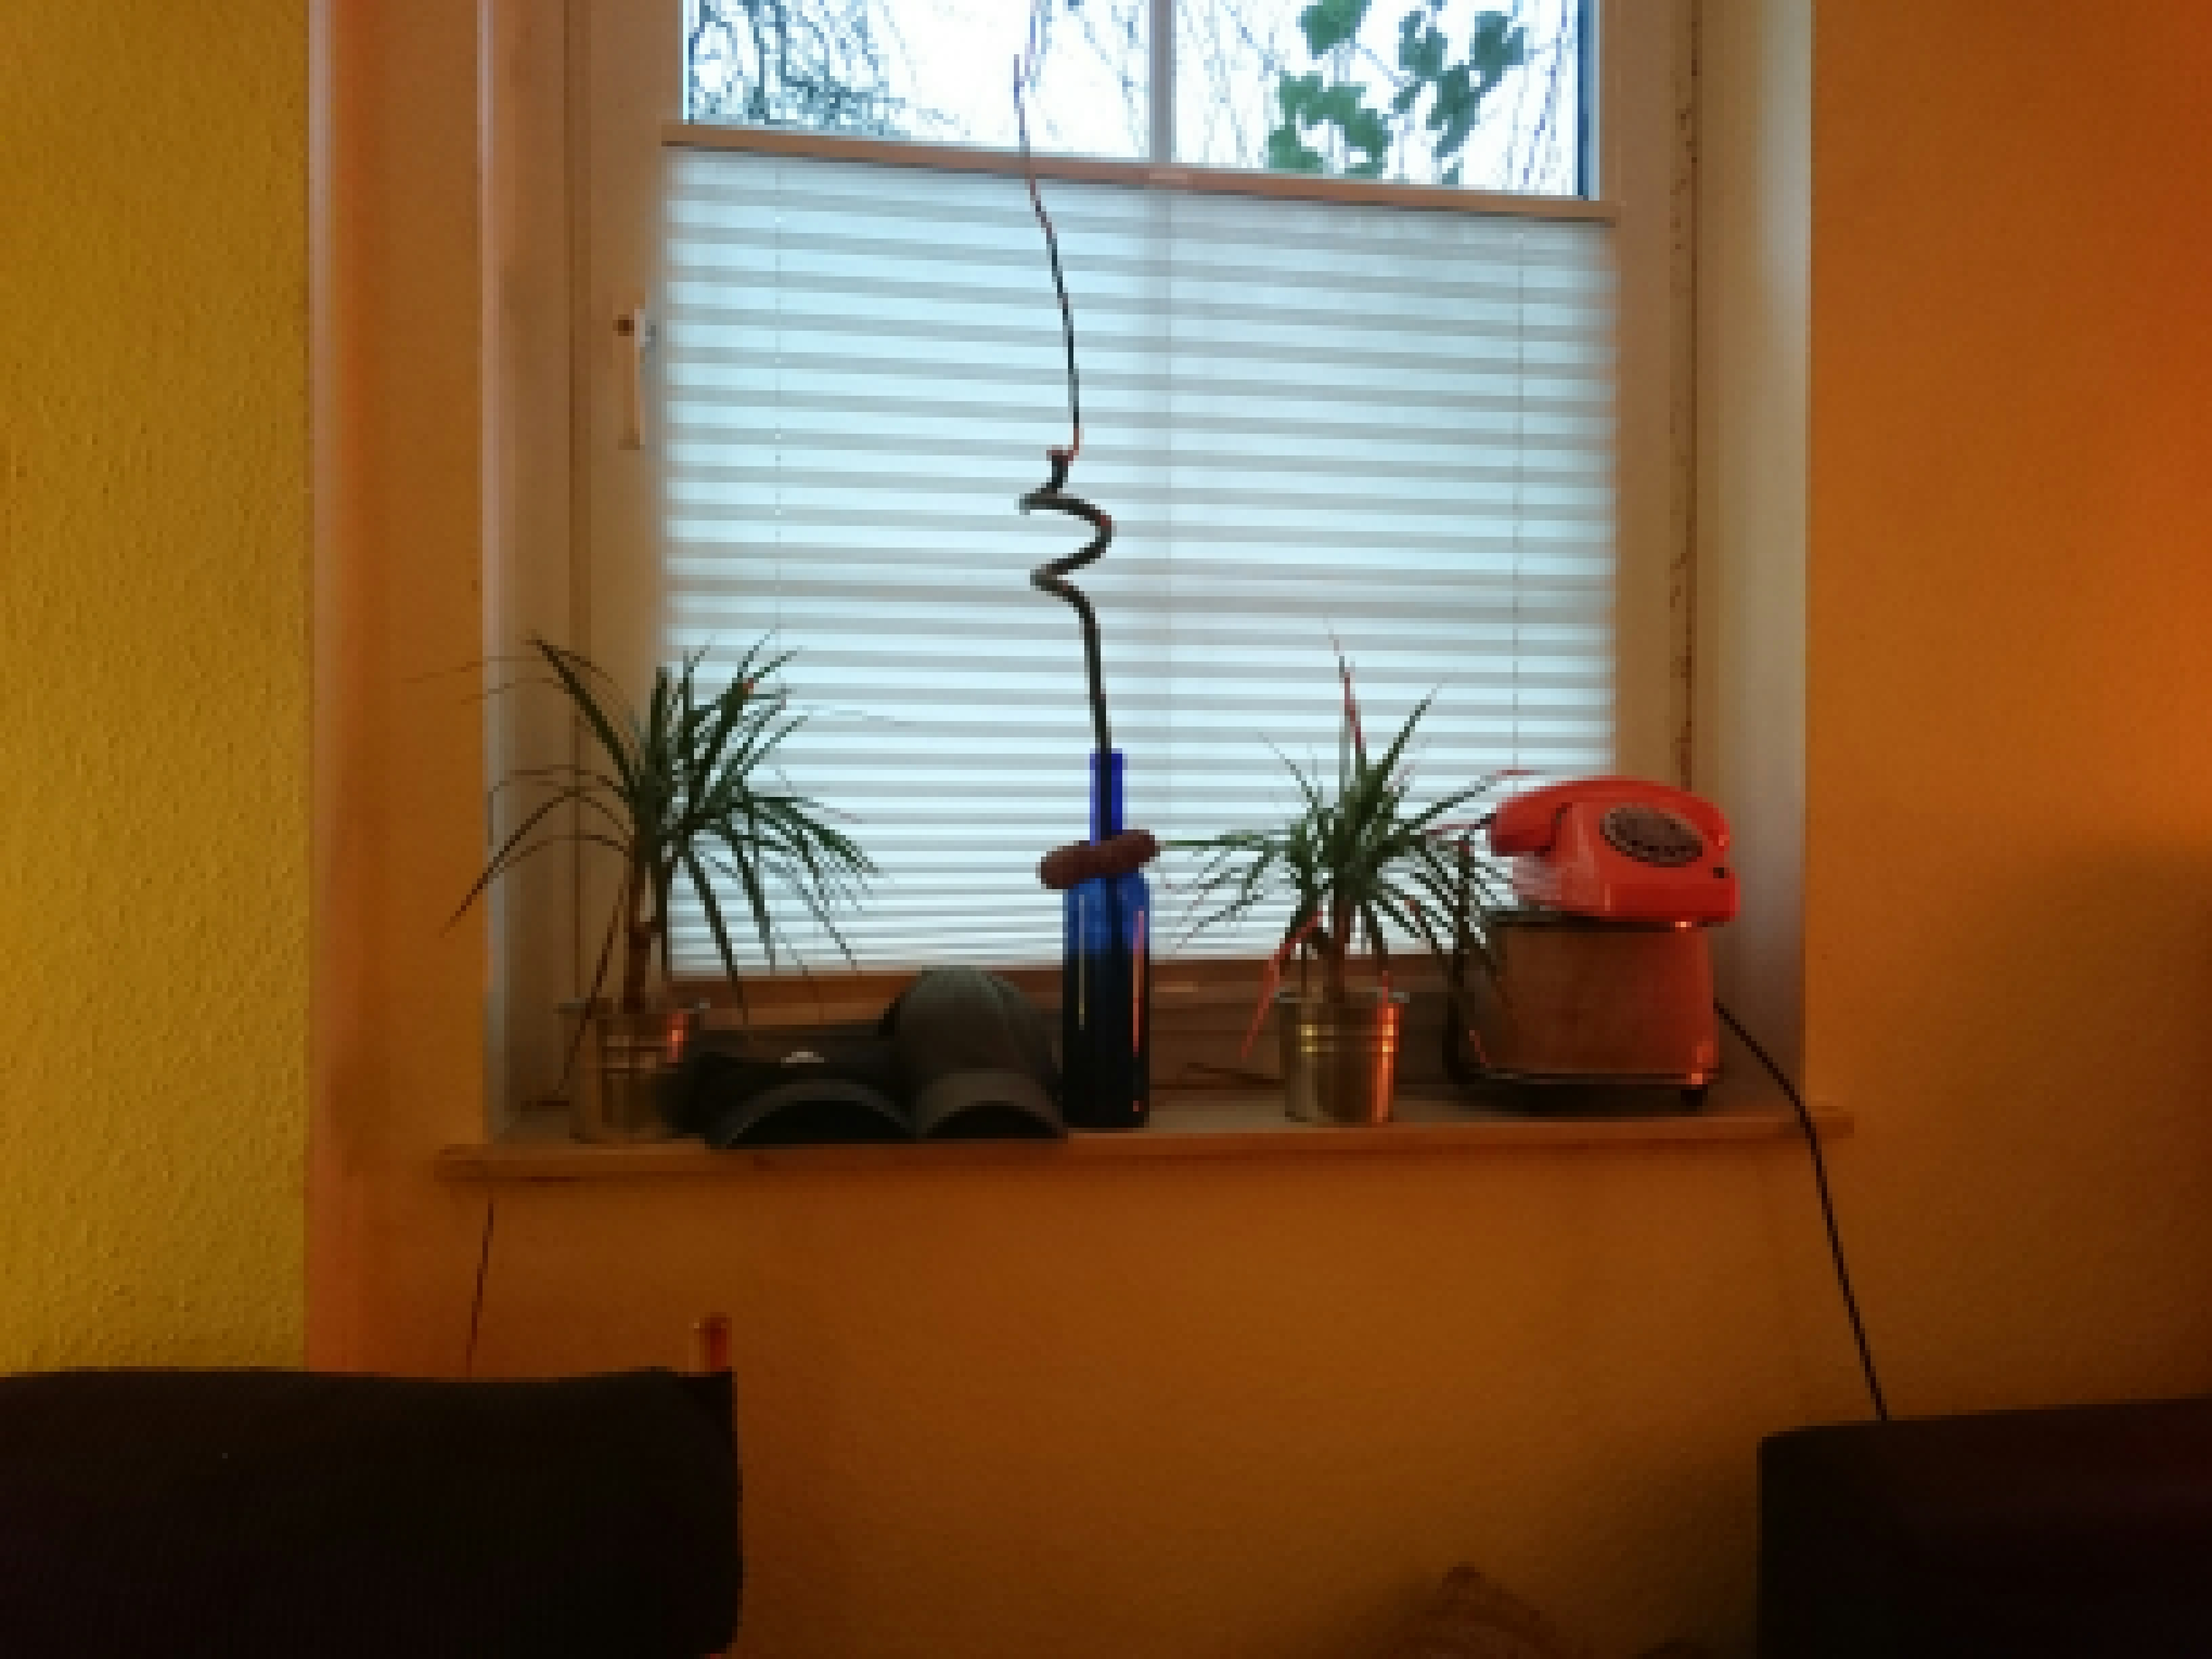
\includegraphics[width=1.4\textwidth]{img/Fotos/QuantiPig_Skalar_8x8.jpg}
	\caption[QuantiPig skalare Quantisierung 8x8 px]{QuantiPig skalare Quantisierung 8x8 px}
	\label{fig:pig_skalar 8x8}
\end{figure}

\begin{figure}[h]
	\centering
		
\includegraphics[width=1.4\textwidth]{img/Fotos/QuantiPig_Skalar_80x80.jpg}
	\caption[QuantiPig skalare Quantisierung 80x80 px]{QuantiPig skalare Quantisierung 80x80 px}
	\label{fig:pig_skalar 8x8}
\end{figure}


\end{landscape}


\clearpage

\subsection{Bildgrößen}
\begin{itemize}
	\item Original: 3,8 MB
	\item skalare Quantisierung:
		\begin{itemize}
			\item 2x2:		3,8 MB
			\item 4x4:		2,6 MB
			\item 8x8:		0,58 MB
			\item 80x80: 	0,12 MB 
		\end{itemize}
	\item Midtread: 4,9 MB
\end{itemize}













\section{Anhang}

